%%%%Draft version
% \documentclass[12pt,letterpaper,spanish,draft,twoside]{book}
%%%%Final version
\documentclass[12pt,letterpaper,spanish,twoside,final]{book}

\usepackage{Thesis}
% New bibliography system: biber (No bibtex needed)
\usepackage[
  backend=biber
]{biblatex}
\addbibresource{bibliografia.bib}

%%%%For producing modified TOC with less space inbetween.
\usepackage{tocloft}
\setlength\cftparskip{-2pt}
\setlength\cftbeforesecskip{1pt}
\setlength\cftaftertoctitleskip{2pt}

%\includeonly{dedicatoria} %Por debug solo compila un capitulo


\begin{document}

\selectlanguage{spanish}

%%%%Change numbering to alphabetic
%\pagenumbering{alph}

%%%%Change numbering to roman
\clearpage \pagenumbering{roman}
%\listoftodos

\begin{titlepage}
\vspace*{-1.5cm}
\noindent\makebox[\textwidth]{%
\begin{tabular}{cc}
\multirow{6}{*}{
\includegraphics[scale=.25]{escudoUNAM.jpg}} \\
\\\\
 & \uuline{\textsc{\large Universidad Nacional Autónoma de México}}\\[.5cm]
 & \textsc{Facultad de Estudios Superiores Acatlán}\\
\\
\\
\end{tabular}}

\vspace{1.5cm}
\noindent\makebox[\textwidth]{%
\begin{tabular}{c@{\hspace{1.5cm}}||@{\hspace{1cm}}lr}
 & \multicolumn{2}{c}{\textsc{\large ``Modelado Gráfico de un Cuerpo}}\\
 & \multicolumn{2}{c}{\textsc{\large Neumático con OpenGL a Base de}}\\
 & \multicolumn{2}{c}{\textsc{\large Ecuaciones Diferenciales''}}\\[1cm]
 & \multicolumn{2}{c}{\textsc{\Large{T \ E  \ S \ I \ S}}}\\[1cm]
 & \multicolumn{2}{c}{\textsc{\large que para obtener el grado de:}}\\[1cm]
 & \multicolumn{2}{c}{\textsc{\large Licenciado en Matemáticas}}\\
 & \multicolumn{2}{c}{\textsc{\large Aplicadas y Computación}}\\[1cm]
 & \multicolumn{2}{c}{\textsc{\Large{P \ R \ E \ S \ E \ N \ T \ A}}}\\[1cm]
 & \multicolumn{2}{c}{\textsc{\Large Jorge Antonio García Galicia}}\\[2cm]
 & \textsc{Director de Tesis:}\\
 & & \textsc{Dr. María del Carmen Villar Patiño\ \ \ \ \ \ \ \ \ \ \ }\\[1.5cm]
 & México, D.F. & 2008
\end{tabular}
}
\end{titlepage}

% \newpage
% \thispagestyle{empty}
% \mbox{}

\cleardoublepage

\thispagestyle{empty}
\vspace*{8cm}
\begin{flushright}
\textit{Para Onatta\\
por estar siempre en mi corazón.}
\end{flushright}                 

% \newpage
% \thispagestyle{empty}
% \mbox{}

\cleardoublepage

\chapter*{Agradecimientos}

{\small
Agradezco al Consejo Nacional de Ciencia y Tecnología (\textsc{conac}y\textsc{t}), por apoyar esta investigación con la beca \textsc{cvu}--266004 para estudios de Maestría en la Universidad Nacional Autónoma de México.

La tesis fué realizada bajo la supervisión de Edgar Garduño, quien me invito a participar en este proyecto. Agradezco enormemente su apoyo, guía y paciencia.

Estoy agradecido con mis sinodales: Jorge Urrutia, Fernando Arámbula, Jorge Márquez y Ernesto Bribiesca, por las importantes recomendaciones, sugerencias y correcciones. Sin duda hicieron que este trabajo mejorara su calidad. 

Agradezco también al Departamento de Ciencias de la Computación del Instituto de Investigaciones en Matemáticas Aplicadas y en Sistemas por permitirme hacer uso de sus instalaciones y por todos los recursos materiales con los que me apoyaron.

Y por supuesto, gracias\ldots

A mi mamá (q. e. p. d.), mi papá y mis hermanos, por siempre haber creído en mi y por haberme apoyado no solo en este trabajo, si no en todos los proyectos que he emprendido en la vida.

A Erika, por las platicas, el apoyo, los momentos compartidos, la solidaridad y por ser la persona tan maravillosa que es.

A Magali, Laura y Jose Luis, mis \emph{roomates}, por haberme permitido compartir su vida y su amistad.

A mi grupo de trabajo: Etna, Fátima, Eduardo, Verena y Cinthya. Por la compañia, por haberme rebotado ideas y por siempre haber estado dispuestos a ayudarme.

A \emph{los inges}: Sergio, Federico y Omar, por haber sido mis compañeros y amigos. Y por haberme apoyado en esos momentos tan difíciles que me tocó pasar. Agradezco también mis compañeros de clase durante la maestría. En especial a Tzolkin, Carlos Alegría, Eliza, Uriel, Marlene, Nahela, Paty, Jaime Cabrera, Toño, Sebastian Bejos y Sonia. Por haberme permitido estudiar a su lado, por todo lo que les aprendí y por su amistad.

A mi amigos: José Raul, Sergio (maría), Jorge (primo), Bernardo, Onatta, Yesenia, Karina, Mariano y Chac. Primero por su amistad, luego por todas las veces que me escucharon y por último por haber tenido siempre tiempo de preguntarme: \emph{¿Cómo va tu tesis?}

A Carmen Villar, por su amistad y por haberme mostrado por primera vez el maravilloso mundo de las gráficas por computadora.

A toda la gente que paga sus impuestos y que cumple con su trabajo en paz.
}
\cleardoublepage

\chapter*{Resumen}
Este trabajo trata de como visualizar campos escalares que han pasado por un proceso de digitalización.
En particular se usa una técnica de graficación por computadora conocida como visualización por superficies o \emph{surface rendering}.

Se asume que se tienen conjuntos digitales de datos que provienen de haber muestreado de manera uniforme el espacio en tres dimensiones.
Asumimos que este muestreo está hecho en una rejilla rectangular y por lo tanto tenemos una imagen digital en 3D o volumen.
Hacemos dos suposiciones importantes sobre el volumen.
Primero, que es una buena aproximación del campo escalar y segundo que no tenemos información de la manera como se realizó la digitalización.

\cleardoublepage
%%%%For changing the title of table of contents
%\renewcommand*\contentsname{}
\tableofcontents
\cleardoublepage
\listoffigures
\cleardoublepage
\listoftables
\cleardoublepage
\listofalgorithms
\cleardoublepage


%%%%Change numbering to arabic
\clearpage \pagenumbering{arabic}

\chapter*{Introducción}
\addcontentsline{toc}{chapter}{Introducción}
\markboth{INTRODUCCIÓN}{INTRODUCCIÓN}

Uno de los retos más constantes en las ciencias de la computación, y en especial del área de graficación por computadora, ha sido el de alcanzar cada vez mayor realismo.
Sin embargo, este objetivo comúnmente se opone al de hacer modelos simples que requieran de poco poder de cómputo.

Es cierto que cada vez tenemos computadoras más poderosas, pero como seres humanos que somos siempre hemos querido muchas cosas más de las que tenemos.
Hoy en día el que una simulación se pueda ejecutar rápidamente en una computadora personal es casi tan importante como el que esa simulación se vea real.

Modelos que se sabe son bastante efectivos, como las ecuaciones de Navier-Stokes, también son computacionalmente muy costosos.
Por lo tanto, no pueden ser ocupados en simulaciones que requieran de alcanzar tiempo real.

Los videojuegos son un claro ejemplo de simulaciones que requieren de una adecuada combinación de realismo y rapidez de ejecución.
Dentro de esta área, se dice que se alcanza tiempo real cuando el programa responde más rápido de lo que el usuario puede darle instrucciones.
El objetivo principal de este trabajo es encontrar un modelo que conjunte el mayor realismo posible, sin olvidar alcanzar \emph{tiempo real}.

Hace tiempo, cuando buscaba algún tema interesante para realizar mi trabajo de titulación, no tenía una idea clara de lo que quería hacer.
Por un lado sabía qué me gustaba de las materias de mi licenciatura, también sabía que quería hacer una tesis que de alguna manera tuviera que ver con el área de gráficas por computadora.

Afortunadamente para mi, eso fue lo único que necesité para que la maestra Carmen Villar se interesara en asesorar mi trabajo de titulación, aun cuando no tenía un tema bien definido.
Después de buscar en diversas fuentes de información llegamos al sitio web de Maciej Matyka, sobre simulación basada en física, en donde pude consultar el artículo~\cite{Matyka:Presion}.
Desde el primer momento este artículo llamó  mi atención, el modelo propuesto gozaba de las tres características más deseables en un modelo de simulación: era sencillo de entender, sencillo de implementar y era visualmente muy agradable.

%%Replantar si este prrafo va
Teníamos entonces una idea de donde comenzar, sólo nos hacia falta un problema que valiera la pena modelar.
Discutiendo en el laboratorio de Linux de la FES Acatlán, quizás un poco inspirados en la película American Beauty, tuvimos la idea del sistema que dio origen al presente trabajo.
Al final creo que el resultado poco tiene que ver con la inmortal escena, pero estoy convencido de que al menos para mí ha sido un camino igual de inspirador.
%% aqui termina

Otra meta que quería alcanzar era utilizar Software Libre en todo este trabajo. 
Sin duda, el utilizar una biblioteca como OpenGL me favoreció para poder alcanzar esta meta, al tratarse de una especificación libre y multiplataforma.
La mayor parte del trabajo fue realizada bajo un sistema GNU/Linux y el texto fue escrito en \LaTeX. Considero que este objetvo fue cumplido.

A lo largo del desarrollo, tanto del programa como del trabajo escrito, me encontré con muchísimos obstáculos.
Algunos se debieron a mi desconocimiento de ciertas áreas de la física, y otros simplemente a mi falta de habilidades de programación.
Sin embargo, estoy convencido que en ambos aspectos este trabajo me ayudó a superarme.

La pregunta más importante que ahora trato de responderme es: ¿a quién le sirve este trabajo?
Indudablemente me sirvió a mí el escribirlo, y quiero pensar que también le servirá a cualquier persona que lo lea.
¿Quién puede ser este lector potencial?
Es un trabajo de animación por computadora, por lo que le debe servir a cualquier persona que desee hacer una animación de cuerpos flexibles.
También creo que es un trabajo que modela adecuadamente las leyes físicas del fenómeno, así que se puede beneficiar de él cualquier persona que desee aprender o enseñar cómo funcionan los cuerpos neumáticos.
Por último, le sirve a cualquier estudiante que busque alguna aplicación de las matemáticas y la física en la animación.

La manera como decidí organizar este trabajo es la siguiente:
%%Aqui nos quedamos
En la primera parte se revisó el marco teórico.
Éste trata principalmente de aquellas partes de la literatura, que aunque ya están escritas, quizás no sean tan obvias para estudiantes de la licenciatura de Matemáticas Aplicadas y Computación.
Este capítulo fue por mucho el más divertido de escribir.

En el siguiente capítulo, ya adentrado en la situación a modelar, traté en mayor detalle las estrategias de implementación del modelo.
Es un capítulo en el que intenté de plasmar, sobre todo, las cosas que me fueron más difíciles en el desarrollo de la investigación y cómo fue que encontré soluciones a ellas.

El tercer capítulo trata de cómo se hizo el programa en C++ para esta simulación. 
Aunque el código que aquí escribo puede ser mejorado de muchas maneras, es una solución que funciona.
Y si bien no me preocupé en optimizar el código, si se ganó un poco de claridad. 
Además, considero dado el  propósito de este trabajo, que la programación no es \emph{tan} importante.

El capítulo final fue por mucho el más gratificante de escribir.
En él presento las pruebas y juegos a los que sometí mi programa una vez que terminé el desarrollo.
Al escribir este capítulo aprendí dos cosas: que siempre hay más cosas que hacer después de que uno piensa que ha terminado algo y que los resultados no siempre son los que uno espera.
De hecho, el desarrollo de esta investigación, de la que fui parte desde su nacimiento, me hizo llevarme unas cuantas sorpresas en su edad madura.

Por último, sólo me queda esperar que los lectores de este trabajo encuentren al leerlo, un poco de la diversión que me dejó a mí escribirlo.


\chapter{Un poco de Matemáticas}
\label{chap:mate}
Sólo para probar el siguiente texto está en ingles: \textenglish{In god we thrust}.

En éste capítulo se presentan varios ejemplos com muchas matemáticas. 
Primero, se puede crear una ecuación simple de la siguiente manera:
\begin{equation}
 \label{eq:elipse}
 \frac{x^{2}}{a^{2}} + \frac{y^{2}}{b^{2}} = 1
\end{equation}
Y podemos hace una referencia a ella en el texto de la siguiente manera: La  ecuación \eqref{eq:elipse} representa una elipse.
Si no queremos que las ecuaciones esten numeradas podemos hacer:
\begin{equation}
 \nonumber
 \binom{n}{k} = \frac{n!}{k!(n-k)!} 
\end{equation}
También se pueden insertar ecuaciones dentro de un párrafo, por ejemplo: $\forall x \in \mathbb{R}$. 
Se pueden poner links a un sitio web de la siguiente manera: 
Para aprender acerca de integrales y sumatorias puedes leer el siguiente \href{https://en.wikibooks.org/wiki/LaTeX/Mathematics#Sums_and_integrals}{wikilibro} o puedes buscarlo en \url{www.google.com}.
Nótese que la segunda forma cambia la fuente del texto.
 
Éste es un ejemplo de una función con casos, como si fuera una \emph{pdf}.
\begin{equation}
 \label{eq:pdf}
 f(y) =
 \begin{cases}
   \frac{1}{25} y & \quad \text{si } 0 \leq y < 5 \\
   \frac{2}{25} - \frac{1}{25} y & \quad \text{si } 5 \leq y < 10 \\
   0 & \quad \text{si } y < 0 \text{ ó } y > 10
 \end{cases}
\end{equation}
Éste es un ejemplo de paréntesis que ajustan su tamaño automáticamente:
\begin{equation}
 \nonumber
 P\left(A=2\middle|\frac{A^2}{B}>4\right)
\end{equation}
Finalmente, pongo un ejemplo de como escribir una serie de pasos matemáticos usando el entorno: \verb|align|.
Poner $*$ dentro del entorno te perimite omitir los números
\begin{align*}
P\left(X \leq 3 \right) &= \int_{0}^{3} \frac{1}{25} y \,\mathrm{d}y \\
     &= \left. \frac{1}{25} \cdot \frac{1}{2} \, y^{2} \right|_0^3 \\
     &= \frac{1}{25} \left( \frac{1}{2} \, 9 - \frac{1}{2} \, 0 \right) =
     \frac{1}{25} \cdot \frac{9}{2} = \frac{9}{50} \approx 0.18 
\end{align*}

 
\chapter{Construcción del algoritmo de simulación}

En este capítulo nos encargaremos de presentar el algoritmo propuesto por Matyka en~\cite{Matyka:Presion}, que es explicado en más detalle en~\cite{Matika:SoftBody}.
Este modelo no es más que la unión de los modelos del capítulo anterior.
Además definiremos el experimento que deseamos realizar para probar el funcionamieto del modelo.

Más adelante en este mismo capítulo, explicaremos cómo se pueden enfrentar ciertos detalles sobre el algoritmo de Matika.

Primero veremos cómo se puede calcular el volumen de un cuerpo en tres dimensiones, explicaremos como se puede tener una idea general, y por qué para ciertas geometrías del cuerpo, se prestan mejor ciertos algoritmos.

Luego nos enfrentaremos al problema de cómo integrar la ecuación de Newton, con métodos numéricos, analizando dos alternativas, y se presentan las que se consideran las mejores maneras de implementar el integrador en código.

Por último analizaremos el problema más difícil de la implementación: las colisiones.
Esto se analiza en dos partes, la manera como se detectan y la respuesta de las mismas.

\section{Diseño del experimento}
\label{descripcion:experimento}
Necesitamos una simulación gráfica (animación) y el principal objetivo será hacer que se \emph{vea} real.

Se quiere modelar un cuerpo neumático.
Para hacerlo partimos de un cuerpo flexible y le ponemos un fluido dentro, en este caso el gas, además queremos una manera de probar cómo es la interacción de éste con otros objetos de la escena. 

Con base en esos requerimientos, diseñe la siguiente situación: se modela una caja cerrada, en la cual su cara superior tiene la característica de ser formada como un cuerpo flexible, las otras cinco caras son rígidas.
Dentro de esta caja se pone el fluido (gas), de manera que ahora tenemos un cuerpo neumático.
Para probar su interacción con otro cuerpo se le deja caer sobre su cara flexible un cuerpo sólido (en este caso una esfera) y se observa el resultado.

Además para poder hacer varios tipos de pruebas se desea que la animación tenga cierta interactividad, es decir que el usuario pueda, en tiempo de ejecución, cambiar algunas opciones tanto de visualización como también algunos parámetros físicos.

Esta simulación es el objetivo principal del trabajo, y el siguiente capítulo está dedicado a cómo se construyó, mientras que en este capítulo se hace énfasis en los detalles teóricos necesarios para escribir el programa.

\section{El algoritmo de simulación de un cuerpo neumático}

Lo primero que debemos de hacer es exponer las condiciones de nuestra simulación de cuerpo flexible. La situación física que deseamos modelar es la de un cuerpo flexible, hueco que contiene un gas.
Por ejemplo imagínese un globo, un colchón de aire, la llanta de un automóvil o una burbuja.
El comportamiento en el que estamos interesados es en un comportamiento cualitativamente parecido al del fenómeno, es decir que al momento de graficarlo y hacer una animación debe verse \emph{parecido} al sistema real.

El valor de poder graficar de manera realista un modelo como éste, radica en el hecho de que hay muchas cosas que se comportan de manera parecida, y al momento de animar una escena donde hay varios de estos objetos, un modelo físicamente más realista sería muy costoso en tiempo de ejecución.

La forma de atacar este problema será hacerlo con un modelo simple.
Imagínese un cuerpo formado por varios puntos unidos entre ellos por resortes.~\footnote{Este modelo es muy socorrido cuando se trata de modelar ropa o tela, se pueden ver ejemplos en el último capítulo de~\cite{FisicaVideojuegos}, que modela una bandera o en~\cite{Vassilev:Ropa} y~\cite{Provot:Ropa}, ambos modelan ropa sobre una persona}
Ahora imagínese que a un cuerpo cerrado formado por esta \emph{tela}, le ponemos dentro una fuente de aire, que le ayuda a mantener su forma más o menos constante durante las deformaciones permitidas por los resortes que lo forman; ésa es la idea principal de nuestro modelo.

En la Figura~\ref{modelo:fig} podemos ver un pequeño esquema del modelo, en este caso es un hexágono en dos dimensiones.
Desde luego, mientras más compleja sea la forma de nuestro modelo, mas difícil será trabajar con él, pero se verá más realista 

\begin{figure}
 \centering
 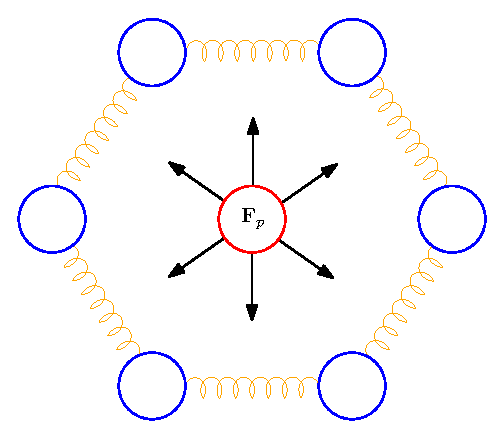
\includegraphics[]{Img/02/modelo}
 \caption[Diagrama del modelo masa, resorte, y presión]{ 
 Un ejemplo de un modelo de masa resorte, con presión. Se trata de un hexágono cerrado, y $\textbf{F}_p$ representa la fuerza debida a la presión.
 } \label{modelo:fig}
\end{figure}

\subsection{Esbozo general del algoritmo}
Una vez conocida la idea, nos empezaremos a preguntar en cómo llevarlo a cabo, es decir cómo podemos implementar este modelo en forma de un algoritmo que seamos capaces de codificar en algún lenguaje de programación.


\begin{figure}
 \centering
 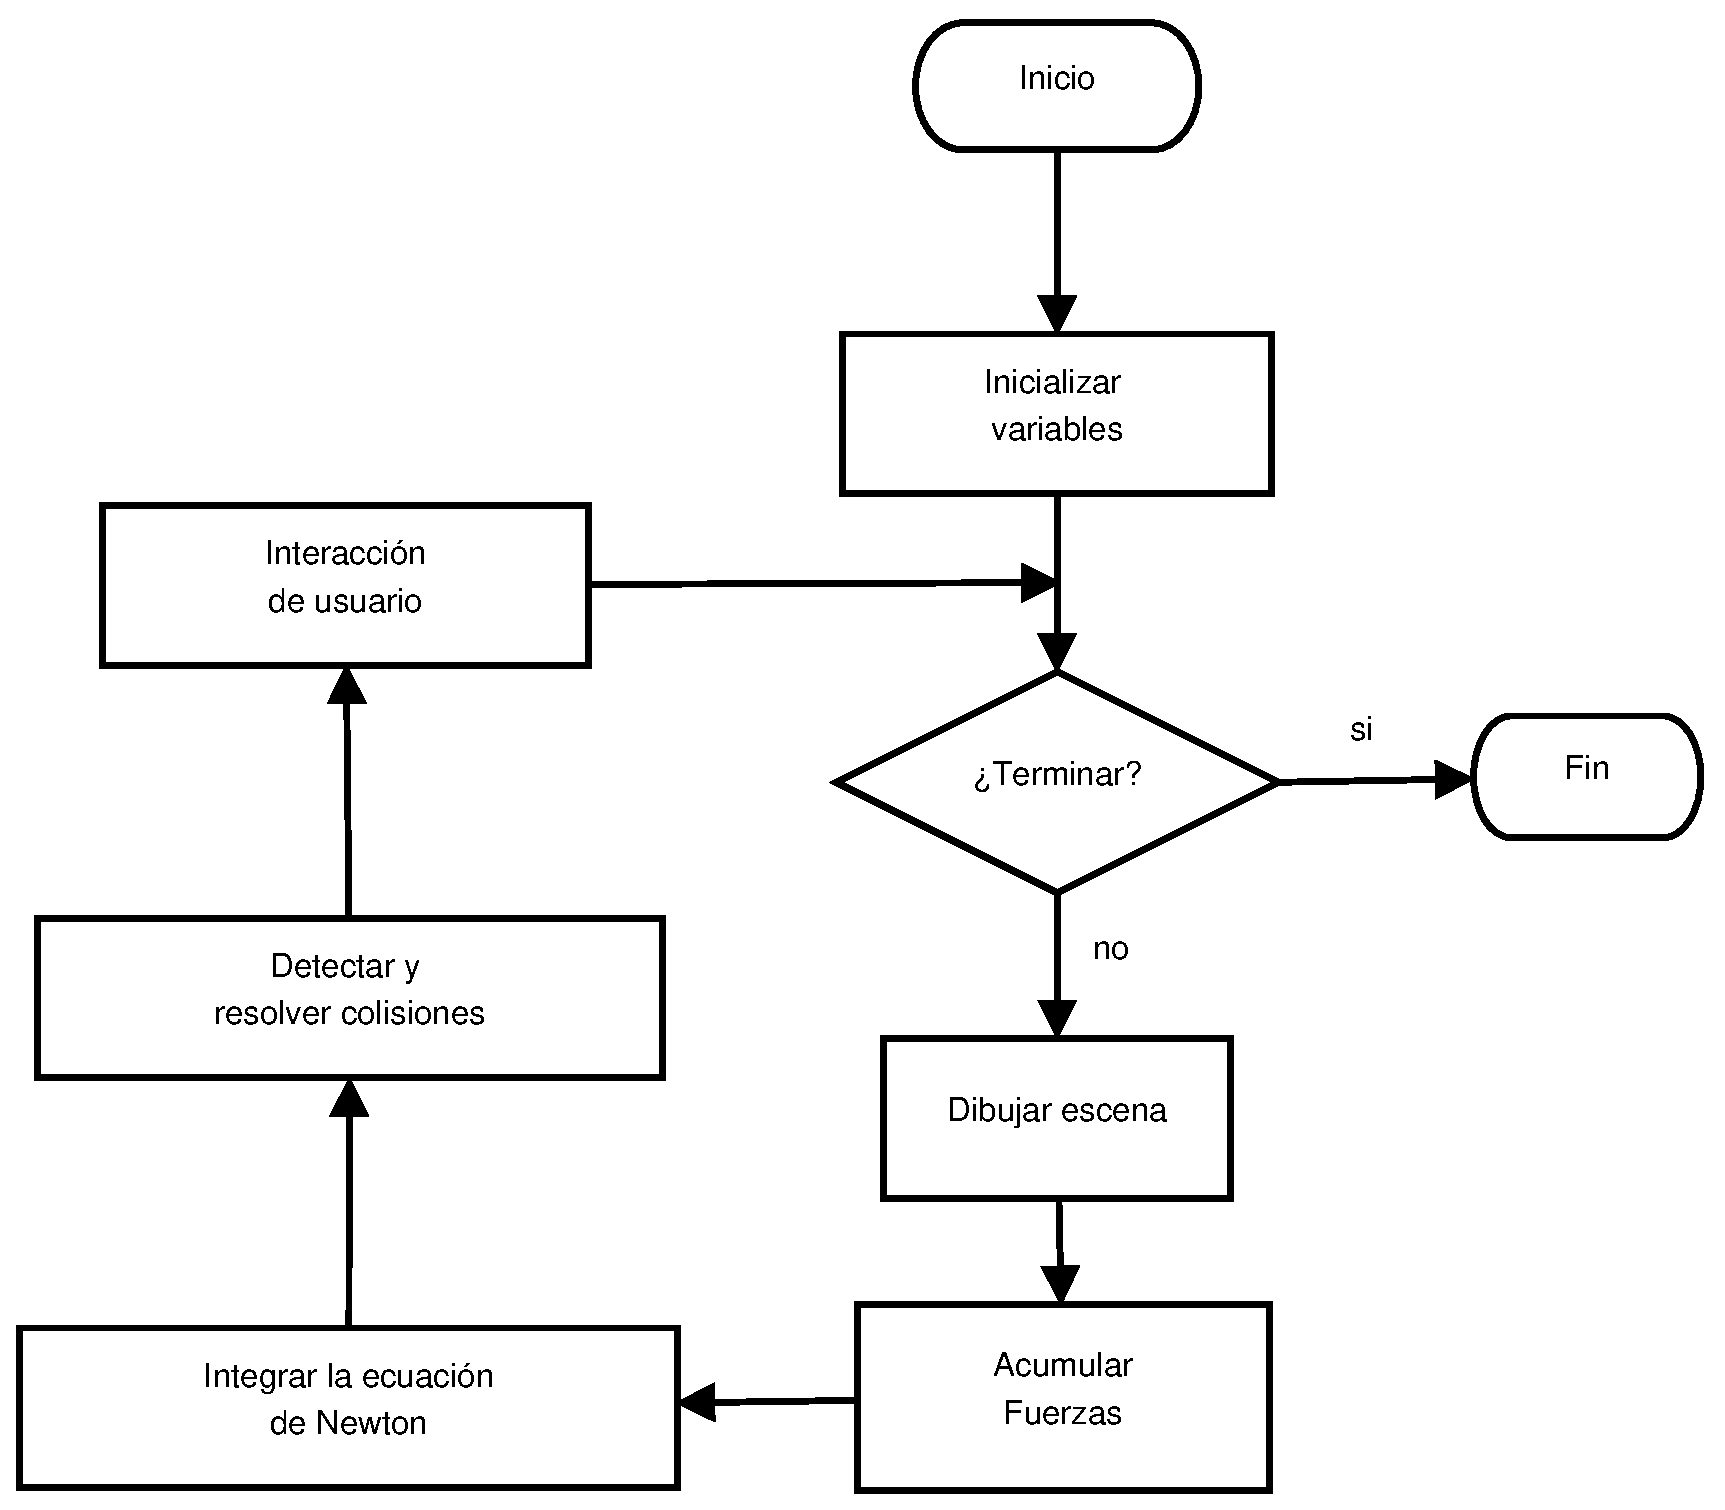
\includegraphics[width=10cm]{Img/02/diagrama_flujo}
 \caption[Diagrama de flujo de la simulación]{ 
 Este diagrama de flujo muestra, los detalles generales a seguir en una animación de un cuerpo flexible. Para cada paso del algoritmo se pueden tener diferentes estrategias, pero en general este esquema no debe cambiar.
 } \label{diagrama_flujo:fig}
\end{figure}

El diagrama de flujo del algoritmo es el que se muestra en al Figura~\ref{diagrama_flujo:fig}, en donde se puede apreciar que sólo se tienen bloques de proceso; cada uno de estos procesos puede ser llevado a cabo de muchas maneras, pero tendrá que ser en este orden, en esta sección veremos con un poco más de detalle cada proceso.

\subsubsection{Inicializar variables}
Lo primero es dar valor a las variables que lo necesiten, me refiero con esto a variables globales, que afectan cómo funciona el programa por el resto de su ejecución.
Dentro de estas variables están los parámetros externos del modelo, es decir esos que no pueden ser calculados dentro del programa y que es necesario que se proporcionen por el usuario.
Lo parámetros necesarios son $m$ para cada partícula, $g$, $k_d$ y $k_s$ para los resortes, $L$ para cada resorte en particular, y $k_p$ para la acumulación de la fuerza debida a la presión.

Otra cosa que debe hacerse en este paso del algoritmo es poner las condiciones iniciales del modelo, por ejemplo, la posición de cada partícula y la velocidad al momento de iniciar la animación.
Y de igual manera con los cuerpos no flexibles que deseemos que interactúen con nuestro modelo, se debe de conocer su posición, si se mueven o no, y cómo van a interactuar con el modelo.

Por último las opciones globales, que afecten a la animación también se deben de obtener aquí, por ejemplo el tamaño del paso $\Delta t$ para mover el modelo, las opciones de los gráficos (si se hará \emph{\foreignlanguage{english}{render}}, o se tratará sólo con el \emph{\foreignlanguage{english}{wireframe}}~\footnote{Cuando sólo se dibujan los bordes de las figuras, como si éstas estuvieran hechas de una malla de alambre se le llama wireframe, cuando dibujamos el área de las figuras y les damos color y efectos de iluminación se dice que se les dio \emph{render}.}) y qué tipo de integrador se ocupará en el modelo.
Alguien me podría decir que estos también son parámetros.
Y en efecto lo son, quise sin embargo hacer la distinción y llamarlos variables globales, por el hecho de que no se deben al modelo en si, sino más bien a la implementación que cada quien haga del mismo, es decir se deben al programa.

\subsubsection{Dibujar escena}
Esta parte del algoritmo debe ser la encargada de dibujar en la pantalla toda la escena.
Para hacer esto debe contar con la información de donde se encuentran cada punto y donde se encuentra cada cosa que queramos dibujar.

Aunque no hay mucho que decir aquí, esta parte es delicada, depende de nuestro conocimiento de las herramientas que vamos a usar para hacer el programa.
Con la ayuda de una biblioteca gráfica, en este caso \emph{\foreignlanguage{english}{OpenGL}}, y los datos necesarios guardados de una manera ordenada, como en una estructura de datos, debemos de ser capaces de implementar esta función.

El detalle de la implementación depende del modelo en cuestión, veré a detalle la que yo use.
Esto puede ser útil para que alguien que deseé implementar una simulación, se de algunas ideas, pero como ya dije, esta parte depende del fenómeno a modelar, por lo que en cada implementación se debe de hacer un análisis.

\subsubsection{Acumular fuerzas}
Las fuerzas que actúan sobre cada partícula del modelo, se pueden identificar como \emph{externas}, es decir que se deben al medio, o \emph{internas} que se deben al cuerpo en sí.
Ejemplos de fuerzas externas son la gravedad, la viscosidad del medio, la resistencia del aire, por mencionar algunas.
Ejemplos de las fuerzas internas son por otra parte: los \emph{resortes amortiguadores} y la debida a la presión del gas.

Cualquiera que sea el caso, en este paso debemos de calcular todas las fuerzas, que intervengan en nuestro modelo, y debemos de acumulársela a cada uno de las partículas que lo conforman, es decir, cada partícula debe tener asociada la suma de todas las fuerzas que actúan sobre ella.
Recordemos que la fuerza en general es un vector, por lo que la acumulación de la que hablo es una suma vectorial de cada una de las fuerzas.

Los detalles de cómo acomular las fuerzas específicas que ocuparé en la simulación se darán en la siguiente sección y con más a detalle en el resto del capitulo.

\subsubsection{Integrar la ecuación de Newton}
Las fuerzas acomuladas en el paso anterior, junto con la posición y velocidad actuales de la partícula, nos proporcionan (como dice la segunda ley de Newton. Ecuación~\ref{ley:Newton}) el siguiente estado, nos dan la información suficiente para saber la nueva posición y la nueva velocidad de la partícula en cuestión. 
Conociendo esto para todas las partículas tendremos determinado el estado completo del modelo en el tiempo siguiente.

Como ésta es una ecuación diferencial, debemos de resolverla, o mejor dicho integrarla, para conocer el siguiente estado del sistema, sin embargo como nuestra acomulación de fuerzas fue hecha a partir de muchas fuerzas, todas ellas de naturaleza distinta, no podremos integrar esta ecuación de manera analítica.
Por esta razón debemos de recurrir a un método numérico que nos permita aproximar la solución.

Por suerte hay muchísimos métodos numéricos que se ajustan a nuestras necesidades, aquí he decidido presentar a dos de ellos solamente, en la sección dedicada a integrar la ecuación de Newton explicaré a detalle cómo funcionan.
De manera general, se puede decir que todos ellos toman como información la posición y velocidad actual de la partícula, el vector fuerza que actúa sobre ella y el instante de tiempo que pasa entre el estado actual y el nuevo estado que queremos calcular (este instante es $\Delta t$).
Y después de hacer cálculos con ellos nos devuelven un nuevo estado, en forma de la nueva posición y la nueva velocidad de la partícula.

\subsubsection{Detectar y resolver colisiones}
En este paso debemos analizar qué pasa cuando nuestro modelo choca o interactúa con otros objetos de la escena.
Estos otros objetos pueden ser cuerpos rígidos como el piso o flexibles como otro cuerpo de la misma característica del nuestro.

El segundo paso es la respuesta a esta colisión.
Este problema es también delicado, pero en general, se va a encargar de ver la partícula que chocó, moverla como respuesta al choque y modificar su estado, es decir su posición y su velocidad.
En una sección posterior de este capítulo hablaré con mas detalle y también daré algunas ideas generales.

\subsubsection{Interacción del usuario}
Este paso es opcional, y depende de si deseamos que la simulación tenga una forma de ejecutarse independiente del usuario o si se desea que éste pueda cambiar la simulación en tiempo de ejecución, por ejemplo modificando algún parámetro de la simulación.

Para enfrentar esto se tiene que recurrir totalmente a la creatividad del programador que vaya a hacer la implementación.
Una buena idea es por ejemplo utilizar alguna biblioteca que exista precisamente para este fin. En éste caso se decidió utilizar un par de bibliotecas que se integran bien con \emph{\foreignlanguage{english}{OpenGL}}.
Por un lado \emph{\foreignlanguage{english}{glfw}}, que permite manejar eventos del ratón y del teclado. 
Y por otro lado \emph{\foreignlanguage{english}{Imgui}} que permite implementar una interfaz gráfica (menú) de usuario.

\section{El sistema de fuerzas}
Es momento de hacernos unas preguntas:
¿Qué es lo que compone nuestro cuerpo?
¿Qué necesitamos saber para implementar este modelo?
La primera pregunta es sencilla: nuestro cuerpo está formado por puntos, que están unidos por resortes, que a su vez se unen para formar las caras.
Resumiendo, nuestro cuerpo es un conjunto de caras, que a su vez son un conjunto de resortes, que a su vez son un conjunto de puntos:
¡Nuestro cuerpo está formado por puntos (partículas)!
La respuesta de la segunda interrogante está ligada a la primera, necesitamos saber todo lo que sea necesario para poder acumular fuerza a las partículas, es decir que para cada una debemos de poder ocupar las ecuaciones~\eqref{fuerzaGravedad}, ~\eqref{fuerzaResorte} y \eqref{fuerzaGas}.

Ciertamente cada una de estas fuerzas es de naturaleza distinta, la fuerza de gravedad es externa y se puede calcular para cada partícula por separado, la de los resortes depende de la posición de cada partícula y de sus vecinos a los cuales está conectado por un \emph{resorte-amortiguador} y por último la de presión depende de la cara en la que esté la partícula y del volumen total del cuerpo.
Podemos resumirlo en el Cuadro~\ref{ejemplo:fuerzas}.

\begin{table}
\ra{1.2}
\begin{center}
\begin{tabular} {@{}llll@{}} 
\toprule
Fuerza & Símbolo &  Parámetros & Datos necesarios \\ 
\midrule
Gravedad & $ \textbf{F}_g $ & $g$, $m$ & Ninguno \\
Resorte & $ \textbf{F}_s + \textbf{F}_d $ & $k_s$, $k_d$ & Partículas unidas por el resorte \\
& & & Velocidad y posición de cada partícula que une el resorte \\
Presión & $ \textbf{F}_p $ & $k_p$ & Partículas que forman la cara \\ 
& & & Volumen total del cuerpo \\ 
& & & Area de la cara \\ 
\bottomrule
\end{tabular}
\end{center}
\caption[Resumen de las fuerzas que actúan sobre cada partícula]{Fuerzas a calcular para cada partícula y que se necesita saber para hacer los calculos}
\label{ejemplo:fuerzas}
\end{table}

Para calcular la fuerza de gravedad es necesario que se conozcan dos parámetros, la masa de cada partícula $m$, y la constante gravitación $g$.
La gravedad debe de acumularse en cada partícula.

La fuerza del \emph{resorte amortiguador} es una fuerza interna.
Para calcularla  necesitamos recibir dos parámetros: $k_s$ y $k_d$.
Luego necesitamos calcular la posición y la velocidad de cada partícula, y saber por cada resorte qué partículas está uniendo.
Cuando tengamos que acumular esta fuerza recorreremos todos los resortes y por cada resorte calcularemos una fuerza, luego la acomularemos en cada unos de los dos partículas a los que este resorte esté conectado.

Por último, para la fuerza debida a la presión, necesitamos un parámetro externo: $k_p$.
Y para poder calcular esta fuerza debemos conocer antes de empezar el volumen total del cuerpo $V$, luego debemos de saber qué partículas pertenecen a cada una de las caras del cuerpo.
Para acumular esta fuerza debemos recorrer cada una de las caras que forman el cuerpo, en cada caso calculamos el área de la cara y acumulamos la fuerza $\textbf{F}_p$ que le corresponda en cada una de las partículas que la forman.

\section{Área, volumen y vectores normales}
Los parámetros necesarios para calcular la fuerza de presión son el volumen total del cuerpo, el área de cada una de las caras, y un vector normal a dicha cara; como ya se dijo, esto depende enteramente de la geometría del cuerpo que se quiera modelar.
Sin embargo, esto no quiere decir que no se puedan dar algunas técnicas generales que en alguna medida puedan ser adaptadas a alguna geometría particular.
El propósito de esta sección es precisamente el de explicar esas técnicas generales.

\subsection{Cálculo de áreas}
Para calcular el área de un cuerpo geométrico generalmente se calcula el área de cada una de sus caras y después se suman.
Empezando por el caso más simple, supongamos que tenemos un triángulo formado por tres puntos, sabemos las coordenadas de cada uno de los puntos, y queremos su área.
Supongamos que los puntos son denotados por $\textbf{P}$, $\textbf{Q}$ y $\textbf{R}$.
Podemos calcular dos de las aristas del tríangulo si calculamos los vectores que van de $\textbf{P}$ a $\textbf{Q}$ y de $\textbf{P}$ a $\textbf{R}$.
Luego podríamos calcular el producto cruz de los dos vectores que acabamos de encontrar y obtener su norma, finalmente la mitad de la norma sería el área del tríangulo que estamos buscando.

$$\overrightarrow{\textbf{PQ}} = \textbf{Q} - \textbf{P}$$
$$\overrightarrow{\textbf{PR}} = \textbf{R} - \textbf{P}$$
$$ A = \frac{1}{2} \vert \overrightarrow{\textbf{PQ}} \times \overrightarrow{\textbf{PR}} \vert$$

Si queremos calcular el área de un cuadrilátero podemos usar la idea anterior y \emph{triangular}, el cuadrilátero en dos partes, supongamos que queremos calcular el área del cuadrilátero formado por los puntos $\textbf{P}$, $\textbf{Q}$, $\textbf{R}$ y $\textbf{S}$, podríamos calcular el área del tríangulo $\triangle \textbf{PQR}$ y luego sumar el área del tríangulo $\triangle \textbf{SRQ}$.
Dicho de otra manera:

\begin{eqnarray} 
A_{T} & = & A_{\triangle \textbf{PQR}} + A_{\triangle \textbf{SRQ}} \nonumber \\
A_{T} & = & \frac{1}{2} \vert \overrightarrow{\textbf{PQ}} \times \overrightarrow{\textbf{PR}} \vert \times \frac{1}{2} \vert \overrightarrow{\textbf{SQ}} \times \overrightarrow{\textbf{SR}} \vert \nonumber \\
\label{formulaArea}
A_{T} & = & \frac{1}{2} \left( \vert \overrightarrow{\textbf{PQ}} \times \overrightarrow{\textbf{PR}} \vert + \vert \overrightarrow{\textbf{SQ}} \times \overrightarrow{\textbf{SR}} \vert \right)
\end{eqnarray}

Este resultado de hecho, puede ampliarse aun más con el enunciado siguiente:

Sea $P$ un polígono simple, sin agujeros, dado por la secuencia ordenada de vértices $\textbf{P}_i = (x_i, y_i)$, $i = 1,\ldots,n$, (por ejemplo en el sentido contrario a las agujas del reloj), entonces el área de $P$ es:
$$A(P) = \frac{1}{2}\sum^{n-1}_{i = 1} \det (\textbf{P}_i, \textbf{P}_{i + 1}) + \frac{1}{2} \det (\textbf{P}_n, \textbf{P}_1)$$

Este teorema fue tomado de \cite{GeometriaParaCAD} donde también es demostrado. 
Con la adecuada combinación de estas técnicas es sencillo ingeniárselas para poder calcular el área de una cara.

\subsection{Cálculo de volúmenes}
Calcular volúmenes es usualmente más complejo que calcular áreas, y por ende casi siempre es computacionalmente costoso, de ahí que además de maneras geométricas de calcular un volumen siempre está la alternativa de aproximar un volumen.
De nuevo hay que pensar que queremos lograr con la simulación si rapidez en la ejecución, o apego a la realidad física.

No hay que olvidar también que para todo modelo y sus respectivos parámetros, siempre hay diferentes grados de sensibilidad, por ejemplo en el caso de nuestro modelo el volumen sólo es utilizado para poder determinar la fuerza escalar de la presión, por lo que es un modelo \emph{poco sensible} al cálculo del volumen.
Es decir, es válido aproximar en este rubro, sin perder mucha realidad en el modelo.

\subsubsection{Volúmenes aproximados}
Hay varias formas de aproximar el volumen de un cuerpo, una de ellas es con cajas envolventes o \emph{\foreignlanguage{english}{bounding boxes}}, la idea es muy simple se trata de aproximar el volumen de un cuerpo complejo mediante el volumen de un cuerpo simple que lo contenga.
Es decir, se aproxima el volumen por medio de poliedros regulares ya sean inscritos o circunscritos, tales que den una buena aproximación del cuerpo cuyo volúmen estamos calculando.

Una forma mas simple es aproximando con un \emph{hexahedro regular} cuyo volumen es $ l \cdot w \cdot h $, o largo por alto por ancho; otra forma geométrica que se usa de manera muy común es el \emph{elipsoide}, cuyo volumen es $ \frac{4\pi}{3} a \cdot   b \cdot  c $, donde $a$, $b$ y $c$, son los largos de sus ejes principales.
\subsubsection{Volúmenes Exactos}
Una técnica muy útil para calcular el volúmen de una malla triangular se puede ver en~\cite{Zhang:volumen}.

La técnica consiste recorrer todas la caras, y en cada una calcular el \emph{volumen orientado} del tetraedro cuya base es la cara triangular y cuya punta es el origen del sistema de referencia.
El signo del volumen (por eso dijimos que es un volumen orientada) depende de si el tetraedo apunta hacia el origen.
Eso quere decir que habrá alguna áreas que sean negativas y otras positivas, la suma de todos los volumenes es el volumen de la malla.

Es importante que al usar esta formula, los triangulos apunten hacia el mismo lado de la malla.
En otras palabras, se deben de definir un orden para los vértices de los triangulos (por ejemplo en contra de las manecillas del reloj) y se debe ser consistente en toda la malla.
En efecto, esta técnica usa una normal a la cara del triángulo para orientar, pero dicha normal esta implicita por el orden de los vértices.

En resumen el volumen del la malla formada por $n$ caras traingulares esta dado por:
\begin{equation}
V = \frac{1}{6} \sum_{i=1}^{n} \textbf{g}_i \cdot \textbf{N}_i
\label{eq:volumen}
\end{equation}

En donde $\textbf{g}_i$ y $\textbf{N}_i$ son el baricentro y la normal del triángulo $i$. Y asumiendo que dicho triangulo tiene vértices en el orden $\textbf{v}_{i}^{1}$, $\textbf{v}_{i}^{2}$ y $\textbf{v}_{i}^{3}$ se pueden calcular de la siguiente manera:

\begin{equation}
\textbf{g}_{i} = \frac{(\textbf{v}_{i}^{1} + \textbf{v}_{i}^{2} + \textbf{v}_{i}^{3})}{3}
\label{eq:baricentro}
\end{equation}

\begin{equation}
\textbf{N}_i = (\textbf{v}_{i}^{2} - \textbf{v}_{i}^{1}) \times (\textbf{v}_{i}^{3} - \textbf{v}_{i}^{1})
\label{eq:normTriag}
\end{equation}

Como ya se dijo, se puede transformar cualquier malla poligonal en una malla triangular subdividiendo cada cara en triangulos.
Por ejemplo, nuestro cuerpo flexible esta formado por caras en forma de cuadriláteros.
Cada cara se puede partir por su diagonal para formar dos triángulos.

\subsection{Vectores normales}
Dado un plano podemos encontrar un vector que le sea normal, sólo necesitamos dos vectores linealmente independientes que se encuentren en el plano y calculando su producto cruz obtenemos un vector normal, es decir en términos mas simples, si conocemos tres puntos del plano y no son colineales, podemos calcular el vector perpendicular a ese plano.

Matemáticemente: dado el triángulo formado por los puntos $\textbf{A}_1 = (x_1, y_1, z_1)$, $\textbf{A}_2 = (x_2, y_2, z_2)$ y $\textbf{A}_3 = (x_3, y_3, z_3)$, un vector normal a este plano, es el vector $\textbf{n}$ que se calcula:

$$ \textbf{n} = \overrightarrow{\textbf{A}_1 \textbf{A}_2} \times \overrightarrow{\textbf{A}_1 \textbf{A}_3}$$

Un hecho muy importante es que si queremos calcular el vector normal a una superficie, podemos calcular los vectores normales a cada vértice de ella y luego promediarlos.
Esto por increíble que parezca funciona y es de hecho la manera como se hacen los cálculos de iluminación en la mayoría de los programas de CAD y de simulación gráfica.

Es decir, si tenemos el polígono de $n$ lados, formado por los puntos $\textbf{P}_1, \textbf{P}_2, \ldots, \textbf{P}_n$, ordenados de alguna manera, por ejemplo en sentido contrario a las manecillas del reloj, y queremos el vector normal a este polígono $\textbf{n}$, calculamos los vectores $ \textbf{v}_1, \textbf{v}_2, \ldots , \textbf{v}_n $, de la forma $\textbf{v}_i = \overrightarrow{\textbf{P}_i \textbf{P}_{i + 1}} \times \overrightarrow{\textbf{P}_i \textbf{P}_{i + 1}} $ para $i = 2, \ldots, n$ y $\textbf{v}_1 = \overrightarrow{\textbf{P}_1 \textbf{P}_2} \times \overrightarrow{\textbf{P}_1 \textbf{P}_n}$, y luego el vector normal $\textbf{n}$ es:

\begin{equation}
\label{formulaVecNormal} 
\textbf{n} = \frac{1}{n} \sum_{i=1}^{n} \textbf{v}_i
\end{equation}

Este hecho es fundamental para nuestros cálculos, tanto de la fuerza debida a la presión, como para la iluminación en el render.
Una demostración se puede encontrar en \cite{GeometriaParaCAD}.

\section{Integrar la ecuación de Newton}
Desde que hay modelos físicos, ha habido interés en la solución numérica de ciertos problemas para los que se sabía de antemano que una solución existía, pero no se contaban con métodos adecuados para encontrarla.
Es por esta razón que nace el análisis numérico, sin embrago no fue hasta que se popularizó el uso de las computadoras que este campo tomó más importancia.

Dentro del análisis numérico, es de nuestro interés la solución numérica de ecuaciones diferenciales.
El problema comienza con una ecuación de primer orden con condición inicial y que cumple las condiciones de existencia y unicidad.

Actualmente, hay muchas maneras de atacar estos problemas, es decir muchas familias de métodos.
Por familia quiero decir cuando alguien propone un método y llega otra persona más y le hace correcciones, ahora hay dos métodos pero en escencia funcionan con la misma idea, por eso son dos métodos de la misma familia.

El primer método para obtener una aproximación numérica de la solución de una ecuación diferencial es el método de Euler, y desde entonces se han propuesto muchísimos métodos e ideas más.
El Cuadro~\ref{historia:metodos} es una línea del tiempo que tiene algunos de los acontecimientos más importantes del desarrollo de esta disciplina.

\begin{table}
\ra{1.2}
\begin{center}
\begin{tabular} {@{}lp{12cm}@{}} 
\toprule
Año & Evento \\ 
\midrule
1768 & Leonhard Euler publica su método, el primero en la historia \\
1824 & Agustin Cauchy demuestra la convergencia del método de Euler, emplea el método de Euler implícito \\
1855 & En una carta escrita por John F. Bashforth, se mencionan por primera vez los metodos de pasos multiples de Couch Adams \\
1895 & Carl Runge publica el primer método de Runge Kutta \\ 
1905 & Martin Kutta describe el popular método de Runge Kutta de orden cuatro \\ 
1910 & Lewis Fry Richardson anuncia su método de extrapolación. \\
1952 & Charles F. Curtiss y Joseph Oakland Hirschfelder acuñan el término \emph{\foreignlanguage{english}{stiff equations}}. \\
1967 & Loup Verlet publica su método, especialmente enfocado a la mecánica de partículas \\ 
\bottomrule
\end{tabular}
\end{center}
\caption[Evolución histórica de los métodos numéricos]{Una línea de tiempo que muestra algunos de los acontecimientos mas importantes para la solución numérica de ecuaciones diferenciales}
\label{historia:metodos}
\end{table}

En escencia estos métodos se encargan de resolver la ecuacion diferencial de la forma:
\begin{eqnarray}
 \frac{d\textbf{y}}{dt} & = &\textbf{F}(t,\textbf{y}) \nonumber \\
 \textbf{y}(t_0) & = & \textbf{y}_0 \label{condicion:inicial}
\end{eqnarray}

Y para hacerlo toman la condición inicial~\eqref{condicion:inicial}, como el primer valor de la solución, con ella calculan un valor aproximado para la solución $\textbf{y}(t)$ en el tiempo $t = t_0 + \Delta t$.
Ahora este nuevo punto de la solución lo llamamos $\textbf{y}_{n}$ y nos ayuda a encontrar un nuevo punto dando otro paso hacia adelante en el tiempo $t = t_0 + 2\Delta t$
Y así sucesivamente, de manera que la salida de nuestro método son una colección de parejas $(t + n \Delta t, \textbf{y}(t + n \Delta t) )$ la primera de ellas es la condición inicial, y de ahí en adelante se trata de aproximaciones de la solución.

Sin embargo nosotros no queremos resolver una ecuación como ésta, deseamos resolver la ecuación~\eqref{ley:Newton}, que es una ecuación diferencial de segundo orden.
Para poder adaptar este problema al método se propone un cambio de variable $\frac{d\textbf{x}}{dt} = \textbf{v}(t)$, por lo que el problema se transforma en resolver un sistema de dos ecuaciones diferenciales.

\begin{eqnarray}
\frac{d\textbf{v}}{dt} & = & \frac{1}{m} \textbf{F}(\textbf{x}, \textbf{v}, t) \nonumber \\
\frac{d\textbf{x}}{dt} & = & \textbf{v}(t) \nonumber \\
\textbf{v}(0) & = & \textbf{v}_0 \nonumber \\
\textbf{x}(0) & = & \textbf{x}_0 \nonumber
\end{eqnarray}

Los métodos siguientes entonces supondrán que sabemos la velocidad y la posición de la partícula en el tiempo $t$, así como la fuerza que actúa sobre ella en este tiempo, con esta última podremos calcular la posición y la velocidad de la partícula en un tiempo posterior $t + \Delta d$.

\subsection{El método de Euler}
Este método fue el primero de todos, de ahí que también sea el más simple, sin embargo aún tiene algunas ventajas el usarlo.
Básicamente el método de Euler nos dice que si tenemos una ecuación de la forma:
$$\textbf{y}'(t) = \textbf{f}(t, y)$$
Con una condición inicial de la forma $\textbf{y}(0)=\textbf{y}_0$.

Entonces podemos aproximar el siguiente punto de la solución con la siguiente fórmula de recurrencia:

$$\textbf{y}_{n+1} = \textbf{y}_n + h\textbf{f}(t_n, \textbf{y}_n)$$

En donde $h$ representa el tamaño del paso en el tiempo hacia adelante es decir $h = \Delta t$.

El método de Euler se puede generalizar para sistemas de ecuaciones diferenciales de tamaño $n$.
Estas generalizaciones se pueden ver en casi cualquier libro de Ecuaciones y en cualquier libro de análisis numérico.
Aquí sólo daré las fórmulas de recurrencia para el caso de $n=2$ por ser el que estamos interesados en resolver.

Dado el sistema:
\begin{eqnarray}
\textbf{x}'(t) & = & \textbf{f}(t, \textbf{x}, \textbf{y}) \nonumber \\
\textbf{y}'(t) & = & \textbf{g}(t, \textbf{x}, \textbf{y})
\label{sistema:general}
\end{eqnarray}
Con las condiciones iniciales:

\begin{eqnarray}
\textbf{x}(t_0) & = & \textbf{x}_0 \nonumber \\
\textbf{y}(t_0) & = & \textbf{y}_0
\label{condiciones:general}
\end{eqnarray}

Entonces la solución se puede aproximar con las siguientes fórmulas de recurrencia:
$$\textbf{x}_{n+1} = \textbf{x}_n + h\textbf{f}(t_n, \textbf{x}_n, \textbf{y}_n)$$
$$\textbf{y}_{n+1} = \textbf{y}_n + h\textbf{g}(t_n, \textbf{x}_n, \textbf{y}_n)$$

Ahora vamos a poner nuestro sistema de manera que podamos ocupar estas fórmulas para resolverlo:
\begin{eqnarray}
\textbf{v}'(t) & = & \frac{1}{m}\textbf{F}(t, \textbf{x}, \textbf{v}) \nonumber \\
\textbf{x}'(t) & = & \textbf{v}(t, \textbf{x}, \textbf{v})
\label{sistema:particular}
\end{eqnarray}

Y nuestras condiciones iniciales son:
\begin{eqnarray}
\textbf{v}(t_0) = \textbf{v}_0 \nonumber \\
\textbf{x}(t_0) = \textbf{x}_0
\label{condiciones:particular}
\end{eqnarray}

Por lo tanto para resolver nuestro sistema con el método de Euler se tiene:

\begin{eqnarray}
\textbf{v}_{n+1} & = & \textbf{v}_n + \frac{h}{m}\textbf{F}(t_n, \textbf{x}_n, \textbf{v}_n)\nonumber \\
\textbf{x}_{n+1} & = & \textbf{x}_n + h\textbf{v}_{n + 1}
\label{formulas:Euler}
\end{eqnarray}

\subsubsection{El error del método de Euler}
Como en todo procedimiento numérico, en el método de Euler se tiene un error, el cual puede encontrarse para nuestro caso por medio de la expansión en la serie de 
Taylor para la función que determina la posición de una partícula.

$$\textbf{x}_{n+1}  =  \textbf{x}_n + h\textbf{v}_n$$
$$\textbf{x}(t_0 + h) = \textbf{x}(t_0) + h \textbf{v}(t_0)$$

Pero sabemos que la serie de Taylor de la trayectoria de una partícula es:

$$\textbf{x}(t_0 + h) = \textbf{x}(t_0) + h \textbf{x}'(t_0) + \frac{1}{2}h^2\textbf{x}''(t_0) + \textbf{O}(h^3)$$

Entonces el error en el método de Euler está dado por la diferencia de ambas expresiones es decir:

$$-\frac{1}{2}h^2\textbf{x}''(t_0) + \textbf{O}(h^3)$$

Este error es el error de truncamiento, o debido al método en sí.
Al momento de implementarlo existe también un error por redondeo, que es debido a que las computadoras operan con un número finito de decimales, sin embargo este error es difícil de estimar y sale del alcance de mi investigación.
De aquí en adelante cuando me refiera al error de un método numérico siempre me referiré al \emph{error por truncamiento}.

\subsubsection{Ventajas y desventajas del método de Euler}

Como todo algortimo este método presenta ventajas y desventajas, éstas se deben tanto al método como a su implementacion en este modelo.
Aquí listaré algunas de ellas.

Ventajas:
\begin{itemize}
\item Se puede implementar fácilmente.
\item Se puede integrar partícula por partícula, dado que sólo requiere de una evaluación de $\textbf{F}$.
\item Es rápido de ejecutarse.
\end{itemize}

Desventajas:
\begin{itemize}
\item Tiende a \emph{explotar} rápidamente.
\item Su error es alto.
\item Es muy sensible a las variaciones pequeñas, por lo que tarda en estabilizarse.
\end{itemize}

\subsection{El método de Runge Kutta}
Supongamos que se tiene una ecuación de la forma
$$\textbf{y}'(t) = \textbf{f}(t, \textbf{y})$$
Con su respectiva condición inicial de la forma $\textbf{y}(0)=\textbf{y}_0$.

El método de Runge y Kutta nos dice que la solución en el siguiente paso de tiempo puede aproximarse con la siguiente fórmula de recurrencia:
$$\textbf{y}_{n+1} = \textbf{y}_n + \frac{h \left(\textbf{k}_{n}^{1} + 2\textbf{k}_{n}^{2} + 2\textbf{k}_{n}^{3} + \textbf{k}_{n}^{4} \right)}{6} $$
 
En donde $h$ representa el tamaño del paso en el tiempo que se desee aproximar y los coeficientes $\textbf{k}_{n}^{1}$, $\textbf{k}_{n}^{2}$, $\textbf{k}_{n}^{3}$, $\textbf{k}_{n}^{4}$ se pueden calcular de la siguiente manera:

\begin{eqnarray}
\textbf{k}_{n}^{1} & = & \textbf{f}(t_n, \textbf{y}_n) \nonumber \\
\textbf{k}_{n}^{2} & = & \textbf{f}(t_n + \frac{h}{2}, \textbf{y}_n + \frac{h}{2} \textbf{k}_{n}^{1}) \nonumber \\
\textbf{k}_{n}^{3} & = & \textbf{f}(t_n + \frac{h}{2}, \textbf{y}_n + \frac{h}{2} \textbf{k}_{n}^{2}) \nonumber \\
\textbf{k}_{n}^{4} & = & \textbf{f}(t_n + h, \textbf{y}_n + h\textbf{k}_{n}^{3}) \nonumber
\end{eqnarray}

Al igual que en el método de Euler, existe una generalización del método de Runge Kutta para poderse ocupar con sistemas de ecuaciones de primer orden.
En casi cualquier libro de ecuaciones se pueden ver estas fórmulas (por ejemplo en~\cite{Blanchard:Ecuaciones}); aquí solo pongo el caso $n=2$ porque es el que voy a ocupar en el modelo.

Supongamos que tenemos de nuevo el sistema~\eqref{sistema:general}, sujeto a~\eqref{condiciones:general}.
Podemos aproximar una solución usando el método de Ruge Kutta con la siguiente fórmula de recurrencia, suponiendo que queremos ir de $t_n$ a $t_{n+1}$.

\begin{eqnarray}
\textbf{x}_{n+1} & = & \textbf{x}_n + \frac{h(\textbf{k}_{n}^{1} + 2\textbf{k}_{n}^{2} + 2\textbf{k}_{n}^{3} + \textbf{k}_{n}^{4})}{6} \nonumber \\
\textbf{y}_{n+1} & = & \textbf{y}_n + \frac{h(\textbf{l}_{n}^{1} + 2\textbf{l}_{n}^{2} + 2\textbf{l}_{n}^{3} + \textbf{l}_{n}^{4}))}{6} \nonumber
\end{eqnarray}

Aquí podemos apreciar que ahora tenemos que encontrar cuatro ponderadores, los $\textbf{k}_{i}^{j}$ y $\textbf{l}_{i}^{j}$ significa que tenemos mas cálculos por hacer.
Los valores de los ponderadores se calculan con las siguientes fórmulas.

\begin{eqnarray}
\textbf{k}_{n}^{1} & = & \textbf{f}(t_n, \textbf{x}_n, \textbf{y}_n) \nonumber \\
\textbf{k}_{n}^{2} & = & \textbf{f}(t_n + \frac{h}{2}, \textbf{x}_n + \frac{h}{2} \textbf{k}_{n}^{1}, \textbf{y}_n + \frac{h}{2}\textbf{l}_{n}^{1}) \nonumber \\
\textbf{k}_{n}^{3} & = & \textbf{f}(t_n + \frac{h}{2}, \textbf{x}_n + \frac{h}{2} \textbf{k}_{n}^{2}, \textbf{y}_n + \frac{h}{2}\textbf{l}_{n}^{2}) \nonumber \\
\textbf{k}_{n}^{4} & = & \textbf{f}(t_n + h, \textbf{x}_n + h\textbf{k}_{n}^{3}, \textbf{y}_n + h\textbf{l}_{n}^{3}) \nonumber
\end{eqnarray}

y

\begin{eqnarray}
\textbf{l}_{n}^{1} & = & \textbf{g}(t_n, \textbf{x}_n, \textbf{y}_n) \nonumber \\
\textbf{l}_{n}^{2} & = & \textbf{g}(t_n + \frac{h}{2}, \textbf{x}_n + \frac{h}{2} \textbf{k}_{n}^{1}, \textbf{y}_n + \frac{h}{2}\textbf{l}_{n}^{1}) \nonumber \\
\textbf{l}_{n}^{3} & = & \textbf{g}(t_n + \frac{h}{2}, \textbf{x}_n + \frac{h}{2} \textbf{k}_{n}^{2}, \textbf{y}_n + \frac{h}{2}\textbf{l}_{n}^{2}) \nonumber \\
\textbf{l}_{n}^{4} & = & \textbf{g}(t_n + h, \textbf{x}_n + h\textbf{k}_{n}^{3}, \textbf{y}_n + h\textbf{l}_{n}^{3}) \nonumber
\end{eqnarray}


El método de Runge Kutta, es mucho más exacto que el método de Euler, de hecho se puede apreciar que el método de Euler, aproxima el siguiente paso con el valor de una pendiente, en cambio el método de Runge Kutta aproxima el siguiente paso con el valor de cuatro pendientes ponderadas, cada una calculada con la aproximación de la anterior.

Supongamos que se tiene de nuevo~\eqref{sistema:particular} sujeto a las condiciones~\eqref{condiciones:particular}, entonces el metodo de Runge Kutta toma la siguiente forma:

\begin{eqnarray}
\textbf{v}_{n+1} & = & \textbf{v}_n + \frac{h}{6}(\textbf{k}_{n}^{1} + 2\textbf{k}_{n}^{2} + 2\textbf{k}_{n}^{3} + \textbf{k}_{n}^{4}) \nonumber \\
\textbf{x}_{n+1} & = & \textbf{x}_n + \frac{h}{6}(\textbf{l}_{n}^{1} + 2\textbf{l}_{n}^{2} + 2\textbf{l}_{n}^{3} + \textbf{l}_{n}^{4})
\label{formulas:RK4}
\end{eqnarray}

Y los ponderadores se pueden calcular de la siguiente manera:

\begin{eqnarray}
\textbf{k}_{n}^{1} & = & \frac{1}{m}\textbf{F}(t_n, \textbf{x}_n, \textbf{v}_n) \nonumber \\
\textbf{l}_{n}^{1} & = & \textbf{v}_n \nonumber \\
\textbf{k}_{n}^{2} & = & \frac{1}{m}\textbf{F}(t_n + \frac{h}{2}, \, \textbf{x}_n + \frac{h}{2}\textbf{k}_{n}^{1}, \, \textbf{v}_n + \frac{h}{2}\textbf{l}_{n}^{1}) \nonumber \\
\textbf{l}_{n}^{2} & = & \textbf{v}_n + \frac{h}{2}\textbf{k}_{n}^{1} \nonumber \\
\textbf{k}_{n}^{3} & = & \frac{1}{m}\textbf{F}(t_n + \frac{h}{2}, \, \textbf{x}_n + \frac{h}{2}\textbf{k}_{n}^{2}, \, \textbf{v}_n + \frac{h}{2}\textbf{l}_{n}^{2}) \nonumber \\
\textbf{l}_{n}^{3} & = & \textbf{v}_n + \frac{h}{2}\textbf{k}_{n}^{2} \nonumber \\
\textbf{k}_{n4} & = & \frac{1}{m}\textbf{F}(t_n + h, \, \textbf{x}_n +h\textbf{k}_{n}^{2}, \, \textbf{v}_n + h\textbf{l}_{n}^{2}) \nonumber \\
\textbf{l}_{n}^{4} & = & \textbf{v}_n + h\textbf{k}_{n}^{3}
\label{ponderadores:RK4}
\end{eqnarray}

\subsubsection{El error del método de Rungue Kutta}
Se puede demostrar por medios algebraicos y de la misma manera que se empleó con el método de Euler que el método de Runge Kutta tiene un error del orden de $\textbf{O}(h^5)$.
Es decir si partimos el intervalo $h$ por la mitad, y damos el doble de pasos el error por truncamiento disminuye en un orden de 16 veces (es decir $\left( \frac{h}{2} \right)^4$, como el error es del orden de $O(h^5)$ se hace $h^4$ veces más exacto).

\subsubsection{Ventajas y desventajas del metodo de Runge Kutta}
Como se puede leer en la bibliografía, el método de Euler y el método de Runge Kutta dependen del tamaño del paso $h$, y se hacen más exactos mientras el paso es más pequeño, pero también se hacen más cálculos, por lo que aumenta la fuente del otro tipo de error, el error por redondeo.
Se acepta de manera general, que de este tipo de métodos, aquel que optimiza esta situación es el método de Runge Kutta de cuarto orden, el método que acabamos de presentar.

Algunas de las ventajas y desventajas para el método de Runge Kutta son las siguientes.

Ventajas
\begin{itemize}
\item Es el método estándar más recomendado y no es tan difícil de implementar (métodos más exactos son considerablemente más difíciles de implementar).
\item Es recomendado por muchos autores y por lo tanto hay mucha documentación.
\item Es rápido de ejecutarse, (Más lento que el Euler, pero para efectos de la animación la diferencia no es apreciable).
\item Es un método muy estable, es muy difícil que explote.
\end{itemize}

Desventajas
\begin{itemize}
\item A diferencia de Euler, requiere de muchas evaluaciones de la función en diferentes puntos (lo que para nosotros significa calcular muchas veces la fuerza sobre la partícula).
\item Las partículas no se pueden integrar por separado, tendrán que integrarse juntas. (todas las que conforman el cuerpo en un solo paso).
\end{itemize}

\section{Cómo enfrentar la colisión de los cuerpos}
Por colisión de los cuerpos entenderemos la manera como lidiar cuando dos cuerpos dentro de la escena quedan en contacto uno con el otro.
Desde nuestro punto de vista esta respuesta se divide en dos pasos: la detección de la colisión y la respuesta a la colisión.

La detección es totalmente un problema geométrico, consiste en que a partir de la información que tenemos de los cuerpos y de la colisión podemos determinar al punto de la colisión y un vector normal a ese punto, este problema es totalmente dependiente de la forma de los cuerpos.
Por el otro lado la respuesta a la colisión es un problema físico y generalmente es más sencillo debido que ya existen algoritmos bien definidos para responder a las colisiones y son independientes de la geometría, es decir son algoritmos generales.

\subsection{La detección de las colisiones}
Como ya se dijo antes la detección de las colisiones es uno de los problemas más complejos que nos podemos enfrentar al hacer una animación.
Básicamente debemos de poder hacer dos cosas aquí: uno, detectar la colisión, es decir mediante una prueba rápida saber si los cuerpos de nuestra escena entraron en contacto, y después ver si podemos determinar un vector normal al punto (o superficie en 3D) de colisión.

Hay básicamente dos tipos de estrategias para resolver este problema, una es por medio de un \foreignlanguage{english}{\emph{bounding volume}}, que se trata de darle la vuelta al problema con una aproximación y otra es por medios estrictamente geométricos es decir tratar de dividir tus cuerpos en figuras de formas elementales, como esferas o paralelepípedos para los cuales las detección es un poco más sencilla.

\subsubsection{Un \foreignlanguage{english}{\emph{bounding volume}}}
Básicamente se trata de imaginar que hay un envolvente de nuestro objeto y este envolvente tiene una forma más sencilla, entonces al probar por la colisión se prueba con el envolvente no con el objeto.
Esto tiene la enorme desventaja de ser una aproximación, por lo que la animación se vera un poco saltada, sin embargo una cuidadosa elección del objeto envolvente hará que este efecto sea mínimo.

Objetos como las elipses, los paralelepípedos y los cilindros son buenos objetos para ser un \foreignlanguage{english}{\emph{bounding volume}}, porque la detección de la colisión es sencilla.

Por ejemplo, en una esfera podemos determinar si un punto esta dentro de ella con tan sólo comparar el cuadrado de su distancia con respecto al centro de la esfera, con el cuadrado del radio. 

Un cilindro con el eje vertical alineado con el eje de la escena es también muy usado.
Si queremos saber si dos objetos contenidos en un cilindro, por ejemplo en un videojuego dos personajes caminando, chocan, sólo debemos ver si la proyección de los ejes principales de los cilindros sobre el eje de la escena (líneas rectas) se interceptan y además las proyecciones de los dos cilindros con el plano $XZ$ (dos círculos) también se intersecan.

Un paralelepípedo o rectángulo, o \foreignlanguage{english}{\emph{bounding box}}, también se usa mucho, por ejemplo cuando la geometría de los objetos hace a la esfera una mala elección, por ejemplo al ver si dos coches chocan en un juego de carreras el rectángulo es una elección mas sabia.

Un rectángulo usado como \foreignlanguage{english}{\emph{bounding box}} generalmente se alinea con las coordenadas del mundo, para así hacer las pruebas de detección triviales, si  por el contrario el rectángulo es alineado con las coordenadas del objeto y este tiene la capacidad de rotar, cada vez que lo haga se necesita volver a calcular el  \foreignlanguage{english}{\emph{bounding box}}.
\subsubsection{Uniendo diferentes geometrías}
Una manera más exacta de predecir si dos objetos de una escena están en colisión, es descomponer la forma completa de un objeto en varios objetos pequeños, y luego probar contra todos los objetos que componen el cuerpo si es que existió la colisión.
Por ejemplo, en el caso de la simulación del cuerpo flexible se podría pensar como que cada partícula que forma el cuerpo es un objeto y luego probar la colisión contra todas las partículas que forman el cuerpo flexible.

Esta técnica es bastante más cara, tanto de implementar como de ejecutarse, sin embargo, da resultados visiblemente más acertados, por ejemplo en un juego de lucha libre, donde la interacción de los luchadores debe de ser bastante creíble, se recomendaría usar este tipo de colisiones.

\subsection{La respuesta de las colisiones}

Como ya habíamos dicho, el trabajo difícil y dependiente de la animación está en la detección de las colisiones, y la respuesta a las colisiones es totalmente física.
Para empezar las colisiones se dividen en dos: elásticas e inelásticas.
La implementación de ambas no se diferencia mucho, aunque sí son diferentes en concepto.

Básicamente en un algoritmo de respuesta de colisiones, se suministran las posiciones y las velocidades de los dos objetos que coliden, más un vector normal unitario al punto de colisión de los dos objetos, o plano normal en el caso de tres dimensiones.
Desde luego que hay dos vectores que cumplen con esa condición, cualquiera de ellos nos servirá siempre y cuando sepamos cual de ellos es el que tenemos.
Ya con esta información debemos ser capaces de responder con dos cosas: una nueva posición de los objetos y una nueva velocidad.

En la Figura~\ref{colision:fig} se ven los diferentes pasos de la respuesta a la colisión de dos círculos.
\begin{figure}
 \centering
  \begin{subfigure}[b]{0.32\textwidth}
    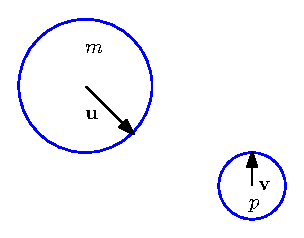
\includegraphics[width=1.2\textwidth]{Img/02/colisionesAntes}
    \caption{Antes de la colisión.}
    \label{fig:coliAntes}
  \end{subfigure}
  \hspace{2cm}
  \begin{subfigure}[b]{0.32\textwidth}
    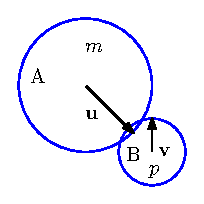
\includegraphics[width=0.75\textwidth]{Img/02/colisionesDetecta}
    \caption{Colisión detectada}
    \label{fig:coliDetecta}
  \end{subfigure}
\\
\vspace{1cm}
  \begin{subfigure}[b]{0.32\textwidth}
    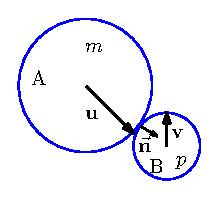
\includegraphics[width=0.8\textwidth]{Img/02/colisionesResponde}
    \caption{Respuesta a la colisión.}
    \label{fig:coliResponde}
  \end{subfigure}
  \hspace{2cm}
  \begin{subfigure}[b]{0.32\textwidth}
    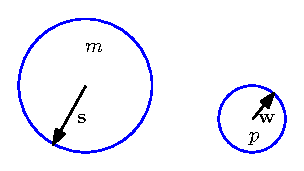
\includegraphics[width=1.1\textwidth]{Img/02/colisionesAjusta}
    \caption{Después de la colisión}
    \label{fig:coliAjusta}
  \end{subfigure}
 \caption[Colisión elástica]{Etapas de detección y respuesta a una colisión} 
 \label{colision:fig}
\end{figure}

\subsubsection{Separar un vector en componentes normal y tangencial}
Antes de explicar la forma en que se responden las colisiones quiero hacer énfasis en la manera como separa un vector en componentes ortogonales (Figura \ref{comVec:fig}), porque es necesario hacerlo en la respuesta a las colisiones.

Para separar a un vector cualquiera $\textbf{v}$ en dos componentes: uno normal $\textbf{v}_n$, y otro tangencial $\textbf{v}_t$ respecto a un vector normal $\textbf{n}$, se hace uso de las siguientes fórmula:

\begin{eqnarray}
\textbf{v}_n & = &\frac{(\textbf{v} \cdot \textbf{n})}{|\textbf{n}|} \frac{\textbf{n}}{|\textbf{n}|} \nonumber \\
\textbf{v}_t & = & \textbf{v} - \textbf{v}_n \nonumber
\end{eqnarray}

Como en los cálculos de detección de colisiones es común que tengamos un vector normal $\vec{\textbf{n}}$, tal que: $|\vec{\textbf{n}}| = 1$, las fórmulas anteriores se simplifican aun más siendo la forma más usada la siguiente\footnote{Las fórmulas~\eqref{eq:sepVector}, se encuentran mal escritas en~\cite{BaraffWitkin:Coursenotes}, y esta fue una de las razones que más me retrasó al momento de hacer este trabajo.}:

\begin{eqnarray}
\textbf{v}_n & = &(\textbf{v} \cdot \vec{\textbf{n}}) \vec{\textbf{n}} \nonumber \\
\textbf{v}_t & = & \textbf{v} - \textbf{v}_n
\label{eq:sepVector} 
\end{eqnarray}

\subsubsection{Colisiones elásticas}

Una colisión elástica es aquella donde el momento y la energía de los objetos, se conservan después de la colisión; son una abstracción que nunca sucede en la vida real.
Aun las colisiones en el espacio exterior son inelásticas aunque están muy cerca de no serlo~\cite{FisicaMatematicasVideojuegos}, pero nos sirven bastante para entender el fenómeno, y en algunos casos son suficientes.
Por ejemplo, pensemos que estamos modelando un juego de billar en 2D una colisión elástica es suficiente.

Supongamos que se tienen dos cuerpos $A$ y $B$, las formas no importan, y sabemos, gracias a un algoritmo de detección de colisiones, que están en colisión y un vector normal $\vec{\textbf{n}}$ a la superficie de colisión.
Suponemos que este vector apunta del cuerpo $A$ al cuerpo $B$ y que es también un vector unitario.

Suponemos también que conocemos todas las propiedades de los cuerpos, es decir su masa, su velocidad y su posición.

Queremos determinar una nueva posición y una nueva velocidad para los objetos como resultado de la colisión entre ellos.
Esto se resumen el Cuadro~\ref{condiciones:Colision}.

\begin{table}
\ra{1.2}
\begin{center}
\begin{tabular} {@{}lll@{}}
\toprule
Objeto & Información conocida & Información por determinar \\
\midrule
$A$ & Masa $m$, Velocidad $\textbf{u}$ & Velocidad ajustada $\textbf{s}$ \\
$B$ & Masa $p$, Velocidad $\textbf{v}$ & Velocidad ajustada $\textbf{w}$ \\
\bottomrule
\end{tabular}
\end{center}
\caption{Condiciones de la respuesta a las colisiones}
\label{condiciones:Colision}
\end{table}

Para entender el porqué de la respuesta a la colisión, es necesario seguir los siguientes pasos\footnote{Esta es una reproducción del procedimiento mostrado en~\cite{FisicaMatematicasVideojuegos} con mi nomenclatura}.
Primero vamos por el caso más simple: dos objetos $A$ y $B$, con velocidades $\textbf{u}$ y $\textbf{v}$ respectivamente chocan, como respuesta a la colisión las velocidades de ambos objetos cambian a $\textbf{s}$ y $\textbf{w}$.
Ver la Figura~\ref{colision:fig}.

Suponemos que: $\textbf{v} = \textbf{0}$. Es decir el cuerpo $B$ no se mueve, está detenido esperando la colisión del cuerpo $A$. Sabemos que tenemos un vector $\vec{\textbf{n}}$ normal al plano de colisión.
Con este vector podemos dividir los demás vectores en una parte normal al plano y otra tangencial  (Figura~\ref{comVec:fig}), es decir:

\begin{figure}
 \centering
 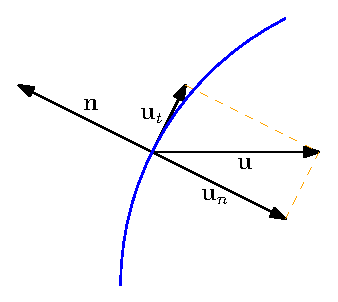
\includegraphics[width=7cm]{Img/02/vector_componente}
 \caption[Separar componente tangencial y normal de un vector]{ 
 El vector $\textbf{v}$ se separa con respecto a $\textbf{n}$ en dos vectores uno normal $\textbf{v}_n$, y uno tangencial $\textbf{v}_t$ 
 } \label{comVec:fig}
\end{figure}

\begin{eqnarray}
 \textbf{u} & = & \textbf{u}_t + \textbf{u}_n \nonumber \\
 \textbf{v} & = & \textbf{v}_t + \textbf{v}_n \nonumber \\
 \textbf{s} & = & \textbf{s}_t + \textbf{s}_n \nonumber \\
 \textbf{w} & = & \textbf{w}_t + \textbf{w}_n \nonumber
\end{eqnarray}

Ahora veamos que es lo qué sabemos de antemano por la forma como planteamos las condiciones del problema: sabemos que: $\textbf{u}_t = \textbf{s}_t$ y $\textbf{v}_t = \textbf{w}_t = 0$, porque esperaríamos que las velocidades sólo se vieran afectadas en su componente normal y porque sabemos que el objeto $B$ estaba inicialmente en reposo.
Así que lo único que necesitamos saber es $\textbf{s}_n$ y $\textbf{w}_n$.

Se sabe también que, como la colisión es elástica, debe de obedecer la ley de la conservación de la energía~\eqref{eq:energia} y la la ley de la conservación de momento~\eqref{eq:momento}.

\begin{equation}
m \textbf{u}_n = m \textbf{s}_n + p \textbf{w}_n
\label{eq:momento}
\end{equation}

\begin{equation}
\frac{1}{2} m \textbf{u}^2 = \frac{1}{2} m \textbf{s}^2 + \frac{1}{2} p \textbf{w}^2
\label{eq:energia}
\end{equation}

Así que tenemos justo las condiciones necesarias para encontrar una solución, pues tenemos dos valores por determinar y dos ecuaciones que las relacionan.
Para encontrar la solución hacemos un cambio de variable $r = \frac{m}{p}$.
Podemos encontrar una expresión para $\textbf{w}_n$ de la ecuación~\eqref{eq:momento}, y lo sustituimos en~\eqref{eq:energia} para obtener el valor de $\textbf{s}_n$. En realidad se obtienen dos valores $\textbf{s}_{n}^{1} = \textbf{u}_n$ y $\textbf{s}_{n}^{2} = \textbf{u}_n \frac{r-1}{r+1}$, tomamos el segundo (el primero corresponde a la condición inicial, por que las colisiones elásticas son reversibles en el tiempo), y lo sustituimos de nuevo en~\eqref{eq:momento} para obtener el valor de $\textbf{w}_n = \frac{2 r \textbf{u}_n}{r + 1}$.

Con esto se tiene todo lo necesario  para resolver una colisión elástica con uno de los dos objetos en reposo. Podemos utilizar el siguiente pseudocódigo:

{\centering
\begin{minipage}{\linewidth}
  \begin{algorithm}[H]
    \caption{Respuesta a una colisión elástica}
    \label{alg:elas}
    \begin{algorithmic}[1] % The number tells where the line numbering should start 0 for no number
\Procedure{RespuestaColisionElastica}{$\textbf{u}, \textbf{n}, m, p$}
\State $r \gets \frac{m}{p}$
\State $\textbf{u}_n \gets$ \Call{parteNormal}{$\textbf{u}, \textbf{n}$}
\State $\textbf{u}_t \gets \textbf{u} - \textbf{u}_n$
\State $\textbf{s}_n \gets \textbf{u}_n \left( \frac{r - 1}{r + 1} \right) $
\State $\textbf{w}_n \gets \textbf{u}_n \left( \frac{2r}{r + 1} \right) $
\State $\textbf{s} \gets \textbf{u}_t + \textbf{s}_n$
\State $\textbf{w} \gets \textbf{w}_n$
\State \Return{$\textbf{s}, \textbf{w}$}
\EndProcedure
\Procedure{parteNormal}{$\textbf{v}, \textbf{n}$}
\State $\textbf{v}_n \gets \frac{(\textbf{v} \cdot \textbf{n})}{|\textbf{n}|} \frac{\textbf{n}}{|\textbf{n}|}$
\State \Return{$\textbf{v}_n$}
\EndProcedure
    \end{algorithmic}
  \end{algorithm}
\end{minipage}
\par
}

En donde la función \verb|parteNormal|, es una función que recibe un vector $\textbf{u}$ y un vector $\textbf{n}$, devuelve la parte normal de $\textbf{u}$ con respecto a $\textbf{n}$.
Es decir, nos sirve para partir al vector $\textbf{u}$ en una parte tangencial y una parte normal a la colisión haciendo uso de las fórmulas \eqref{eq:sepVector}.

Ahora veamos el caso más general, donde $\textbf{v} \neq 0$. Aquí vamos a ocupar el principio de relatividad y le restamos a todo el sistema $\textbf{v}$, lo que lo transforma en el caso anterior. Resolvemos como lo habíamos hecho antes y luego le sumamos a todo el sistema $\textbf{v}$. El pseudocódigo es casi idéntico:
 
{\centering
\begin{minipage}{\linewidth}
  \begin{algorithm}[H]
    \caption{Respuesta a una colisión elástica con ambos cuerpos en movimeinto}
    \label{alg:elasmov}
    \begin{algorithmic}[1] % The number tells where the line numbering should start 0 for no number
\Procedure{RespuestaColisionElastica}{$\textbf{u}, \textbf{v}, \textbf{n}, m, p$}
\State $r \gets \frac{m}{p}$
\State $\textbf{u} \gets \textbf{u} - \textbf{v}$
\State $\textbf{u}_n \gets$ \Call{parteNormal}{$\textbf{u}, \textbf{n}$}
\State $\textbf{u}_t \gets \textbf{u} - \textbf{u}_n$
\State $\textbf{s}_n \gets \textbf{u}_n \left( \frac{r - 1}{r + 1} \right) $
\State $\textbf{w}_n \gets \textbf{u}_n \left( \frac{2r}{r + 1} \right) $
\State $\textbf{s} \gets \textbf{u}_t + \textbf{s}_n + \textbf{v}$
\State $\textbf{w} \gets \textbf{w}_n + \textbf{v}$
\State \Return{$\textbf{s}, \textbf{w}$}
\EndProcedure
    \end{algorithmic}
  \end{algorithm}
\end{minipage}
\par
}

Con esto podemos programar un función general que resuelva colisiones elásticas, sólo debemos asegurarnos de que la función que detecta las colisiones le informe a aquella función de tres cosas: las propiedades del objeto $A$, las propiedades del objeto $B$ y un vector normal al plano de colisión que vaya de $A$ a $B$.

\subsubsection{Colisiones inelásticas}
En una colisión inelástica se tienen un pérdida de energía como respuesta al impacto.
En la realidad las colisiones son inelásticas, podemos apreciar parte de la pérdida de la energía, al escuchar el sonido de la colisión.
Por ejemplo en el billar.

Para simular un colisión inelástica, vamos también a hacer una suposición: que los objetos tiene una cierta eficiencia, y que ésta se mantiene fija para todas las colisiones que involucren ese objeto.
Es una gran simplificación porque en la realidad la eficiencia de una colisión depende de muchos factores, como el medio ambiente, o la velocidad de los objetos al momento de la colisión.

Si dos objetos chocan y uno de ellos tiene \emph{coeficiente de restitución} de 0.9 y el otro un coeficiente de restitución de 0.85, la energía total después de la colisión seria: $\left( \text{0.9} \cdot \text{0.85} \right) \left(  E_b + E_a \right)$.
Donde $E_a$ y $E_b$ es la energía de cada objeto antes de la colisión.
Como se puede ver, el coeficiente de restitución es una manera de medir la \emph{eficiencia} y significa que el primer objeto después de una colisión transmite por ejemplo el 95 por ciento de su energía.

Para resolver una colisión inelástica se usa el mismo procedimiento que en la sección anterior, sólo que ahora la ecuación~\eqref{eq:energia}, toma la siguiente forma:
\begin{equation}
 \frac{1}{2} e m \textbf{u}^2 = \frac{1}{2} m \textbf{s}^2 + \frac{1}{2} p \textbf{w}^2
 \label{eq:energiaIne} 
\end{equation} 

Donde $e$ es el producto de los coeficientes de restitución de ambos objetos. Y se procede de la misma manera que en el caso anterior a calcular los valores de $\textbf{w}_n$ y $\textbf{s}_n$. Resolviendo el sistema formado por las ecuaciónes~\eqref{eq:momento} y~\eqref{eq:energiaIne}.

Las nuevas soluciones son: 
\begin{eqnarray}
\textbf{s}_n & = & \frac{-r\textbf{u} - \sqrt{r^{2} \textbf{u}_{n}^{2} - \left( r + 1\right)  \left( (r - e) \textbf{u}_{n}^{2} + (1 -e) \textbf{u}_{t}^{2} \right) } } { r + 1} \nonumber \\
\textbf{w}_n & = & r \left(  n \textbf{u}_n - \textbf{v}_n \right) \nonumber
\end{eqnarray}

Y el pseudocódigo, que resuelve la colisión de manera inelástica es el siguiente:

{\centering
\begin{minipage}{\linewidth}
  \begin{algorithm}[H]
    \caption{Respuesta general a una colisión inelástica}
    \label{alg:inelas}
    \begin{algorithmic}[1] % The number tells where the line numbering should start 0 for no number
\Procedure{RespuestaColisionInelastica}{$\textbf{u}, \textbf{v}, \textbf{n}, m, p, E_a, E_b$}
\State $r \gets \frac{m}{p}$
\State $e \gets E_a \cdot E_b$
\State $\textbf{u} \gets \textbf{u} - \textbf{v}$
\State $\textbf{u}_n \gets$ \Call{parteNormal}{$\textbf{u}, \textbf{n}$}
\State $\textbf{u}_t \gets \textbf{u} - \textbf{u}_n$
\State $ d \gets r^{2} \left(  \textbf{u}_n \cdot \textbf{u}_n \right) - \left( (r - e) (\textbf{u}_n \cdot \textbf{u}_n) + (1 - e) (\textbf{u}_t \cdot \textbf{u}_t) \right) $
\State $\textbf{s}_n \gets \textbf{n} \left( \frac{ \sqrt{d} - r \textbf{u}_n }{r + 1} \right) $
\State $\textbf{w}_n \gets r \left( \frac{\textbf{u}_n - \textbf{v}_n}{r + 1} \right) $
\State $\textbf{s} \gets \textbf{u}_t + \textbf{s}_n + \textbf{v}$
\State $\textbf{w} \gets \textbf{w}_n + \textbf{v}$
\State \Return{$\textbf{s}, \textbf{w}$}
\EndProcedure
    \end{algorithmic}
  \end{algorithm}
\end{minipage}
\par
}


\chapter{Implementación del modelo}
Este capítulo está dedicado a cubrir los detalles de la implementación del modelo en código, concretamente en lenguaje C++.

Dado que la principal finalidad de este trabajo es el modelado físico, no entraré en detalles en otras áreas del programa más que las que tienen que ver con lo descrito en los capítulos anteriores.

El programa completo contiene módulos para la graficación en \href{http://www.opengl.org/}{OpenGL}, para la interfaz de usuario por medio de \href{https://github.com/ocornut/imgui}{dear imgui}, para la lectura y escritura de imágenes usando \href{http://freeimage.sourceforge.io/}{freeimage} (para cargar texturas y para hacer capturas de pantalla) e implementa el modelo de iluminación de \href{http://en.wikipedia.org/wiki/Phong_reflection_model}{Phong} en shaders por medio de \href{http://www.khronos.org/opengl/wiki/OpenGL_Shading_Language}{GLSL}.

El lector interesado puede consultar el código fuente completo del programa que se incluye en un CD o puede descargarlo de \href{http://github.com/nemediano}{github}.
Aunque el código está escrito en inglés (por ser el estándar) traté de ser lo más extenso en los comentarios en todo el código.
Por lo que el lector que cuente con los conocimientos de programación y graficación por computadora adquiridos en la licenciatura podrá entender y usar todo el código fuente del programa sin ningún problema.

Se decidió implementar el programa usando el paradigma de programación orientada a objetos. 
En la primera sección se describen las clases más importantes: las necesarias para representar las estructuras del modelo y la clase que lleva a cabo la ejecución del programa.

La siguiente sección se revisa cómo se implementaron en código los métodos numéricos usados para integrar la ecuación de Newton.

En la tercera sección se explican las rutinas de la física del modelo, concretamente las rutinas que se encargan de aplicar las fuerzas que intervienen en el modelo.

En la última sección del capítulo, se explica cómo es que se implementaron la rutina tanto de detección como de respuesta a las colisiones.

\section{Diseño de clases}

Decidí usar de la biblioteca de algebra para graficos: \href{http://github.com/g-truc/glm}{glm} por dos razones.
Primero, por que cuenta con tipos de datos para representar vectores en 2 y 3 dimensiones e implementa las operaciones usuales entre ellos.
Y segundo, por que esta biblioteca tiene un alto nivel de integración con OpenGL al grado de ser casi un estandar.

La parte fundamental del modelo la constituyen las partículas; de cada una de éstas nos interesa saber básicamente cuatro cosas: su posición, su velocidad, la fuerza que se le está aplicando y la masa.
Adicionalmente, por un detalle particular a nuestra implementación, se necesita saber si una partícula esta fija.
Si una particúla esta fija, entonces se deben de ignorar las operaciones de integración.
Los métodos nos permiten editar y consultar estos cinco miembros. En este sentido la clase \mintinline{cpp}{Particle} es muy simple~\footnote{En el argot del lenguaje \href{http://www.java.com/en/}{Java} diriamos que la clase \mintinline{cpp}{Particle} es casi un \href{http://en.wikipedia.org/wiki/JavaBeans}{bean}}.

Para representar a los resortes-amortiguadores se creó la clase \mintinline{cpp}{SpringDamper} que tiene como miembros \emph{referencias} a las dos partículas que une éste resorte.
Hago énfasis en que usaremos referencias, pues las partículas van ser usadas para formar varios objetos y se requiere que no sea necesario actualizar en cada objeto por separado cada que una partícula sea modificada. Finalmente, se debe saber la longitud $L$ del resorte cuando está en su estado de reposo.

La clase \mintinline{cpp}{SpringDamper} tiene un define los métodos para:
\begin{itemize}
 \item Actualizar qué partículas forman éste resorte.
 \item Consultar y modificar $L$.
 \item Consultar las posiciones de las partículas que forman este resorte.
 \item Acumular la fuerza del resorte en sus dos partículas dados $k_s$ y $k_d$.
\end{itemize}

La última clase que define el cuerpo neumático es la clase \mintinline{cpp}{Face}, que representa una cara del cuerpo flexible.
Como es de esperar, dado que las caras son cuadriláteros, esta clase solo necesita como propiedades referencias a cuatro partículas.

Adicionalmente, la clase \mintinline{cpp}{Face} implementa los siguientes métodos:
\begin{itemize}
 \item Los accesores y mutadores a las partículas que la forman.
 \item Un método para actualizar las partículas que forman esta cara (equivalente al de \mintinline{cpp}{SpringDamper}).
 \item Un método para calcular el área de esta cara.
 \item Un método que sirve como auxiliar en el cálculo del volumen de todo el cuerpo flexible. La lógica de este método se explica en la Sección~\ref{sec:fuerzaGas}. Aunque ésta no es una propiedad de la cara, por razones de Ingeniería de Software (IS) era conveniente incluirlo en esta clase.
\end{itemize}

También se define una clase para representar el cuerpo flexible: \mintinline{cpp}{SoftBody}.
Esta clase es la más importante de la aplicación.
Y el resto de éste capítulo está dedicado a explicar como funcionan sus métodos.
En este momento, es relevante decir que esta clase contiene una colección de partículas, una colección de resortes y una colección de caras.
Las caras y resortes en realidad contienen referencias a las partículas, de esta manera la información de las partículas sólo está almacenada una vez.

Por orden, esta clase también define una estructura: \mintinline{cpp}{SoftBodyParameters} que contiene todos los parámetros físicos del cuerpo flexible. 
 
Finalmente, se necesita también una clase para representar el único cuerpo rígido en la escena.
La clase \mintinline{cpp}{Ball} tiene como miembros una partícula, un escalar que representa el radio de la esfera y un miembro para registrar qué método numérico se usa para integrar (De nuevo por IS, era conveniente que cada objeto en la escena llevará registro de que integrador está en uso).

La relación entre estas clases esta resumida en el diagrama de clases mostrado en la Figura~\ref{clases:fig}. De nuevo hago énfasis en que la implementación de hecho contiene mas miembros que los mostrados, pues solo aparecen en el diagrama los relevantes para este trabajo.

\begin{figure}
 \centering
 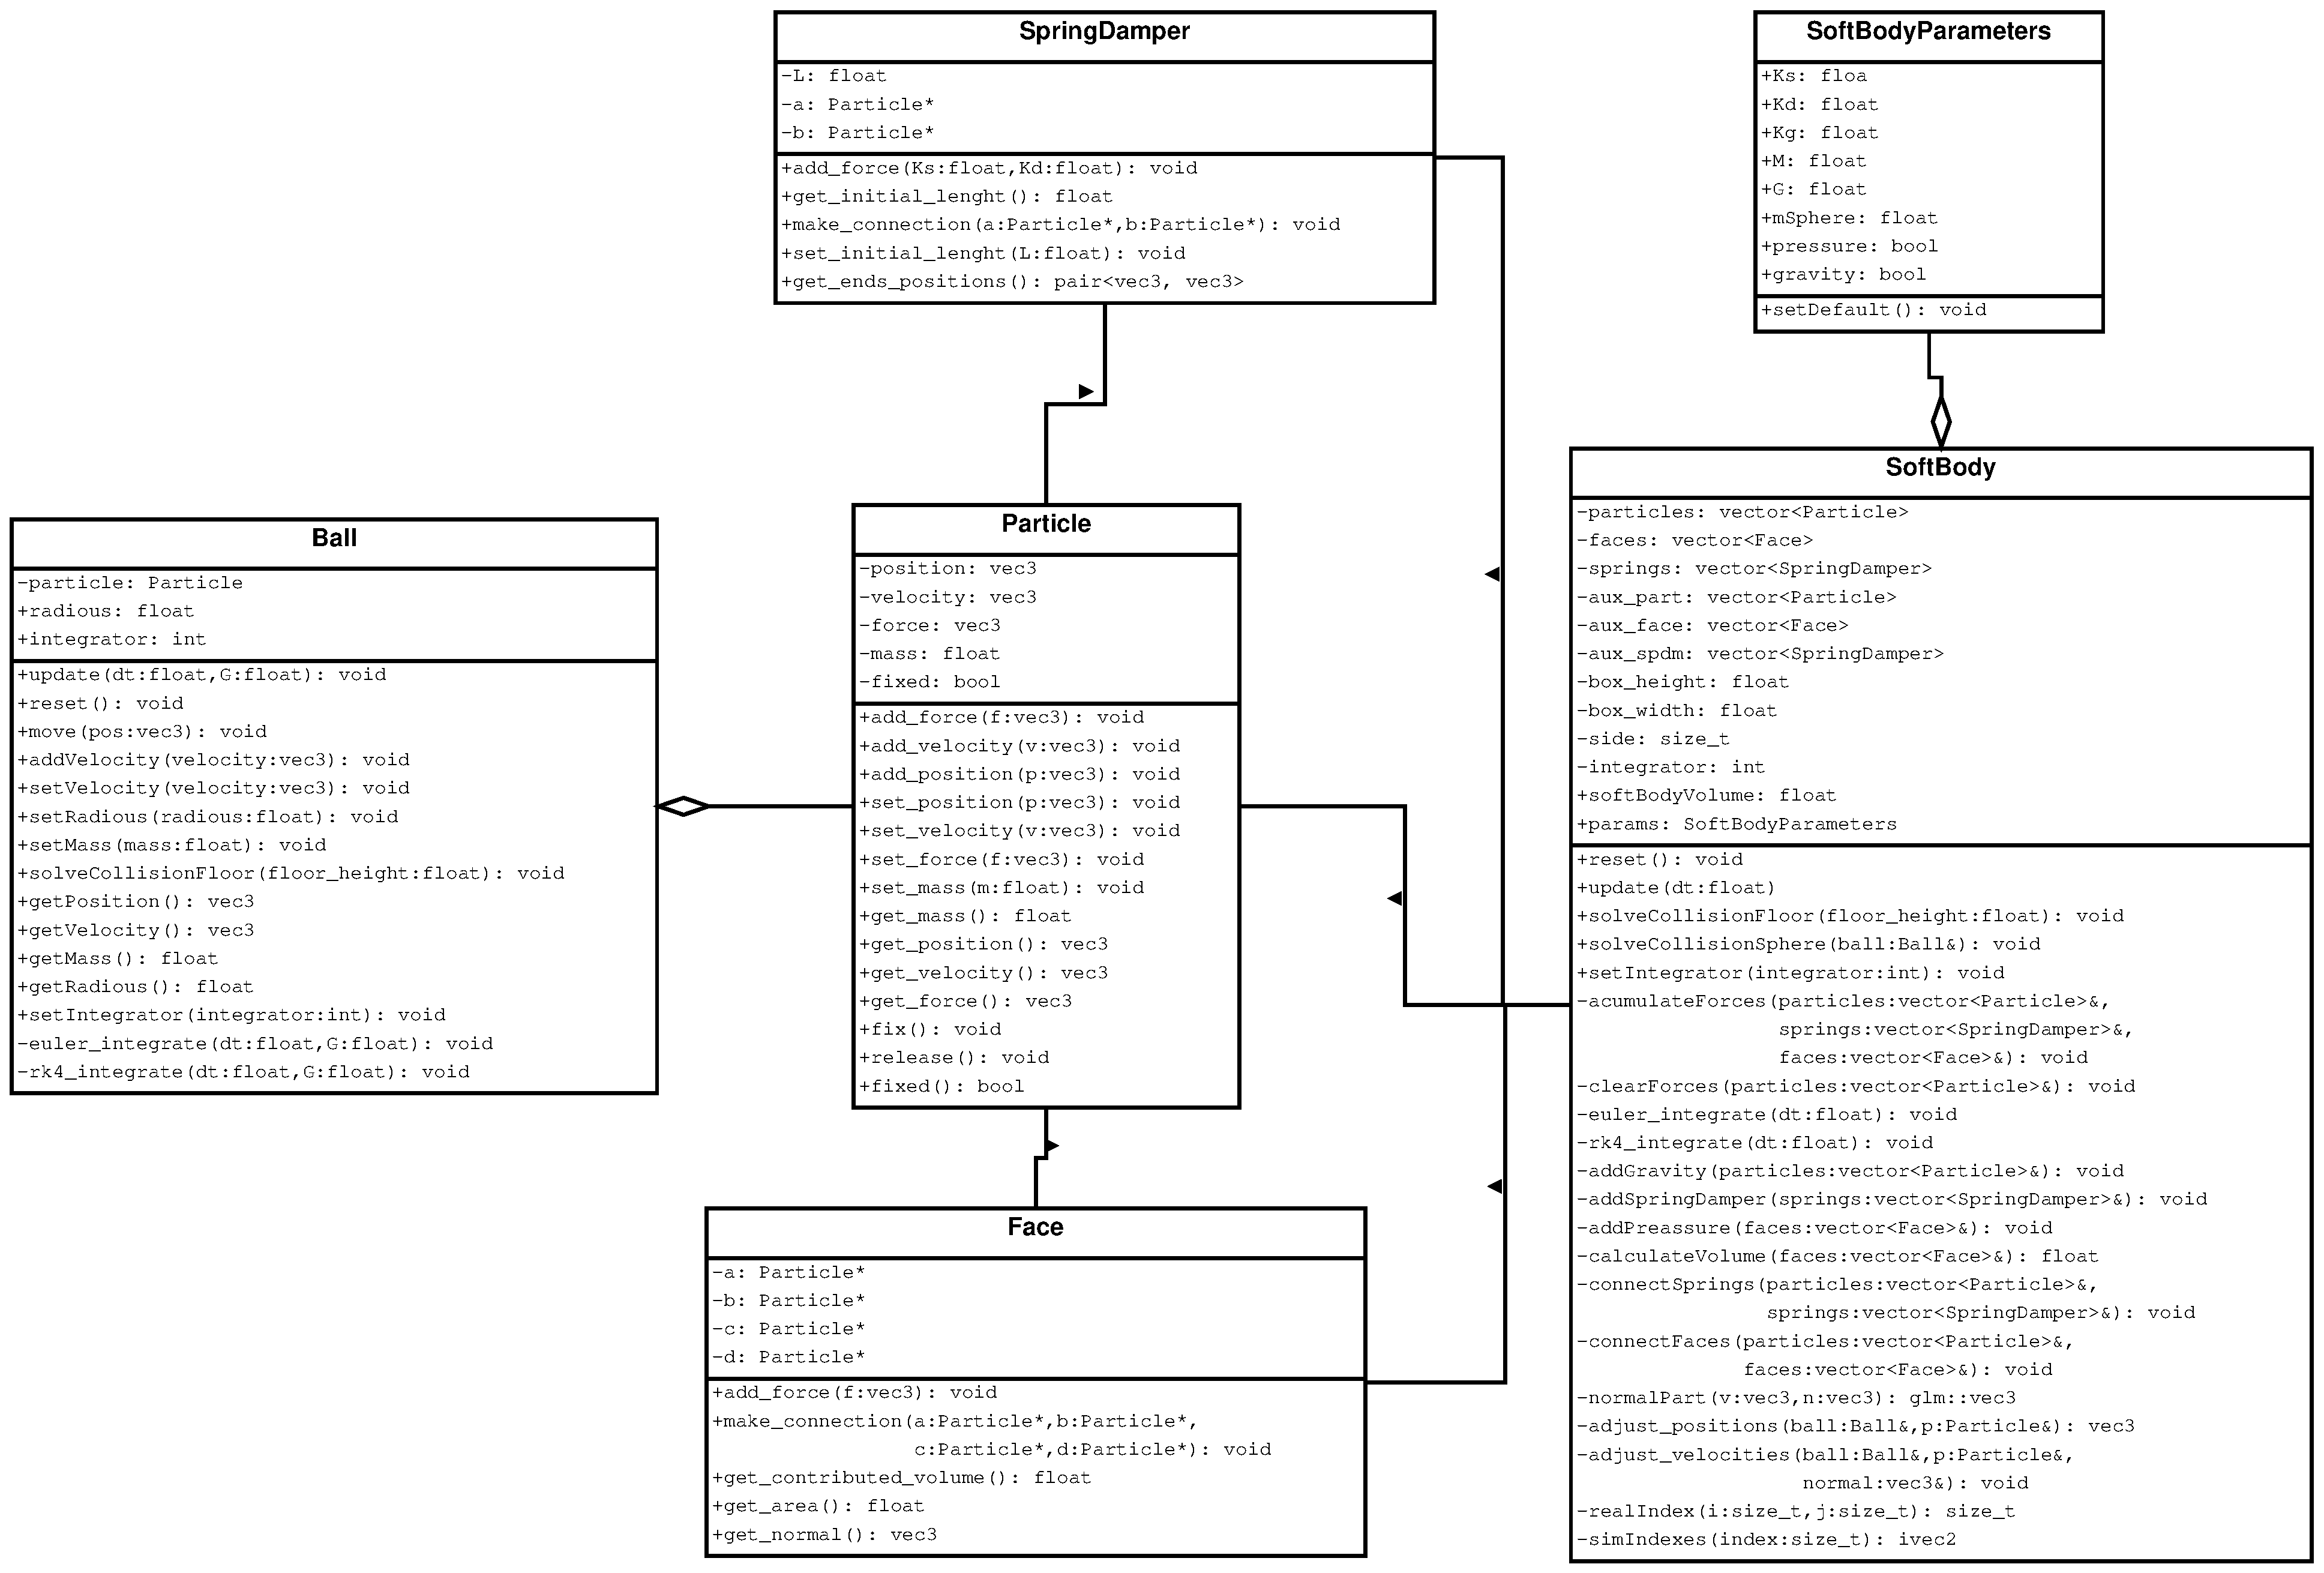
\includegraphics[width=\textwidth]{Img/03/diagramaClases}
 \caption[Diagrama de clases]{ 
 La clase \mintinline{cpp}{Particle} es la unidad de construcción. La clase \mintinline{cpp}{SoftBody} es la que controla la ejecución. 
 } \label{clases:fig}
\end{figure}

\section{Creación del cuerpo flexible}

Cómo se dijo en la sección anterior, hay tres colecciones que forman el cuerpo flexible: las particulas, los resortes y las caras. Estas colecciones estan almacenadas en vectores que forman parte de la clase \mintinline{cpp}{SoftBody}.

Hay algunas cosas que decir aquí: primero, que lo que se quiere modelar es una tela cuadrada que servirá como cuerpo flexible, por lo que el número de partículas es en realidad $n^{2}$ en donde $n$ es el número de puntos en cada lado de la tela (en el código es el miembro \mintinline{cpp}{size_t m_side} de \mintinline{cpp}{SoftBody}), y como no hay resortes en las orillas de la tela el número de resortes totales es $2 (n - 1) (n - 2)$ y el número de caras es: $(n-1)^{2}$.
Segunda, que, pese al arreglo cuadrado de la tela, los puntos son guardados en un arreglo unidimensional (lineal), esto por que simplifica y hace mucho más generales las rutinas de acumulación de fuerza.

Dado que la partículas están en un arreglo unidimensional se hace uso del método \mintinline{cpp}{simIndexes} que recibe el índice de la particula en el vector unidimensional y nos regresa los indices $(i, j)$ que la partícula tendría en un arreglo bidimensional. El metodo \mintinline{cpp}{realIndex} hace la operacion inversa.

La rutina que inicializa las partículas es la siguiente:
\begin{mintedCode}
\inputminted[
  frame=lines,
  framesep=0.25cm,
  baselinestretch=1,
  fontsize=\scriptsize,
  firstline=306, %If you omit this two fields, the whole file is pulled
  lastline=328
  ]{cpp}{../../../GLSamples/SoftBody/physics/SoftBody.cpp}
  \caption{Este es un extracto del método \mintinline{cpp}{recreate_particles} de \mintinline{cpp}{SoftBody}}\label{lst:recreate_particles}
\end{mintedCode}

% \begin{listing}
%   \inputminted[
%   xleftmargin=1.5cm,  %without this option line number goes wrong
%   frame=lines,
%   framesep=0.5cm,
%   baselinestretch=1,
%   fontsize=\scriptsize,
%   linenos,
%   firstline=306, %If you omit this two fields, the whole file is pulled
%   lastline=328
%   ]{cpp}{../../../GLSamples/SoftBody/physics/SoftBody.cpp}
%   \caption{Este es un extracto del método \mintinline{cpp}{recreate_particles} de \mintinline{cpp}{SoftBody}}
%   \label{lst:recreate_particles}
% \end{listing}

El código mostrado en el Listado~\ref{lst:recreate_particles} inicializa la velocidad, la fuerza y la masa de la partículas (la posición es inicializada con una rutina muy simple que esta fuera de la clase \mintinline{cpp}{SoftBody}). También se encarga de fijar las partículas que estan en las orillas de la tela.

La rutina que inicializa los resortes es ejecutada después de las particulas. Se muestra un extracto en el Listado~\ref{lst:connectSprings}.

\begin{mintedCode}
\inputminted[
  frame=lines,
  framesep=0.25cm,
  baselinestretch=1,
  fontsize=\scriptsize,
  firstline=345, %If you omit this two fields, the whole file is pulled
  lastline=368
  ]{cpp}{../../../GLSamples/SoftBody/physics/SoftBody.cpp}
  \caption{Este es un extracto del método \mintinline{cpp}{recreate_particles} de \mintinline{cpp}{SoftBody}}\label{lst:connectSprings}
\end{mintedCode}

Por las condiciones que definimos en nuestra tela. 
\begin{itemize}
 \item Las partículas que están en las arístas superiores e inferiores no tienen un resorte horizontal entre ellas.
 \item Las partículas que están en las arístas izquierda y derecha no tienen un resorte vertical entre ellas.
\end{itemize} 

El algoritmo, pregunta si esta particula puede ser unida (por un resorte) con la partícula a su derecha, de ser así las conecta. Después, pregunta si debe ser unida con la particula abajo de ella, de ser así tambien es conectada.

La logica para formar las caras se presenta en el Listado~\ref{lst:connectFaces}: 
\begin{mintedCode}
\inputminted[
  frame=lines,
  framesep=0.25cm,
  baselinestretch=1,
  fontsize=\scriptsize,
  firstline=372, %If you omit this two fields, the whole file is pulled
  lastline=389
  ]{cpp}{../../../GLSamples/SoftBody/physics/SoftBody.cpp}
  \caption{Este es un extracto del método \mintinline{cpp}{recreate_particles} de \mintinline{cpp}{SoftBody}}
  \label{lst:connectFaces}
\end{mintedCode}

Esta rutina es muy parecida a la anterior: recorre todas las particulas, si la partícula actual, tiene un partícula a su izquierda y otra partícula abajo, entonces se pueden tomar cuatro partículas (pues debe existir otra una partícula en diagonal) para formar una cara.

\section{La física del modelo}
Toca el turno de ver las rutinas que tienen que ver con la acumulación de fuerzas en el modelo.
Como se ha dicho antes hay básicamente tres fuerzas que se deben acumular, la de la gravedad, la de los resortes amortiguadores y la debida a la presión del gas.

Aquí es donde empezaremos a notar el porqué de la construcción de los demás vectores de referencias.

\subsection{La fuerza de gravedad}
La primera y más sencilla de las fuerzas que vamos a poner es la de gravedad.
Como se dijo desde la ecuación~\eqref{fuerzaGravedad}, sólo depende de dos cosas de la masa del objeto y de la constante de gravedad, y además sólo afecta en un componente vectorial el componente $y$, del vector fuerza.

La fuerza de gravedad se aplica a cada una de las partículas del cuerpo flexible. 
Convenientemente, tenemos un vector con dichas partículas.
Por lo anterior y gracias a que glm sobrecarga los operadores en vectores de la manera natural, la implementación es trivial como se puede ver en el Listado~\ref{lst:addGravity}.
La constante de gravedad es un miembro de \mintinline{cpp}{SoftBody} y tiene el signo negativo.

\begin{mintedCode}
\inputminted[
  frame=lines,
  framesep=0.25cm,
  baselinestretch=1,
  fontsize=\scriptsize,
  firstline=584, %If you omit this two fields, the whole file is pulled
  lastline=590
  ]{cpp}{../../../GLSamples/SoftBody/physics/SoftBody.cpp}
  \caption{El método \mintinline{cpp}{addGravity} de \mintinline{cpp}{SoftBody}}
  \label{lst:addGravity}
\end{mintedCode}

\subsection{La fuerza de los resortes}

La implementacion de estos metodos tambien es trivial gracias a nuestro diseño.
Tan solo se debe iterar por todos los resortes de \mintinline{cpp}{SoftBody} en cada resorte se debe ocupar la ecuación~\ref{fuerzaResorte}, para acumular la fuerza en los dos puntos que son unidos por ese resorte (Listado~\ref{lst:addSpringDamper}).
Solo por completez, en Listado~\ref{lst:add_forceSD} se muestra el método \mintinline{cpp}{add_force} de \mintinline{cpp}{SpringDamper} que en escencia implementa la ecuación~\ref{fuerzaResorte}.

\begin{mintedCode}
\inputminted[
  frame=lines,
  framesep=0.25cm,
  baselinestretch=1,
  fontsize=\scriptsize,
  firstline=592, %If you omit this two fields, the whole file is pulled
  lastline=596
  ]{cpp}{../../../GLSamples/SoftBody/physics/SoftBody.cpp}
  \caption{El método \mintinline{cpp}{addSpringDamper} de \mintinline{cpp}{SoftBody}}
  \label{lst:addSpringDamper}
\end{mintedCode}

\begin{mintedCode}
\inputminted[
  frame=lines,
  framesep=0.25cm,
  baselinestretch=1,
  fontsize=\scriptsize,
  firstline=19, %If you omit this two fields, the whole file is pulled
  lastline=32
  ]{cpp}{../../../GLSamples/SoftBody/physics/SpringDamper.cpp}
  \caption{El método \mintinline{cpp}{add_force} de \mintinline{cpp}{SpringDamper}}
  \label{lst:add_forceSD}
\end{mintedCode}

\subsection{La fuerza del gas}
\label{sec:fuerzaGas}

La siguiente fuerza en ser acumulada es la fuerza debida a la presión del gas. Para esto se ocupa la ecuación~\ref{fuerzaGas}, y se debe de acumular una vez por cada cara.
Para poder calcular esta fuerza se necesitan hacer varias operaciones importantes: calcular el volumen total del cuerpo flexible y además calcular el área y el vector normal de cada una de las caras (Listado~\ref{lst:addPreassure}).

\begin{mintedCode}
\inputminted[
  frame=lines,
  framesep=0.25cm,
  baselinestretch=1,
  fontsize=\scriptsize,
  firstline=598, %If you omit this two fields, the whole file is pulled
  lastline=606
  ]{cpp}{../../../GLSamples/SoftBody/physics/SoftBody.cpp}
  \caption{El método \mintinline{cpp}{addPreassure} de \mintinline{cpp}{SoftBody}}
  \label{lst:addPreassure}
\end{mintedCode}

La clase \mintinline{cpp}{Face} implementa la mayoria de las operaciones.

Para hacer el calculo de volumen se hace uso de la ecuación~\eqref{eq:volumen}.
Hay que recordar que el cuerpo flexible esta formado por seis caras.
Cinco de las cuales estan fijas y otra es la tela (o tapa) que es el cuerpo flexible.
El Listado~\ref{lst:calculateVolume} muestra la lógica. La función \mintinline{cpp}{tethVolume} implementa las ecuaciones~\eqref{eq:baricentro} y~\eqref{eq:normTriag}.

\begin{mintedCode}
\inputminted[
  frame=lines,
  framesep=0.25cm,
  baselinestretch=1,
  fontsize=\scriptsize,
  firstline=608, %If you omit this two fields, the whole file is pulled
  lastline=643
  ]{cpp}{../../../GLSamples/SoftBody/physics/SoftBody.cpp}
  \caption{El método \mintinline{cpp}{calculateVolume} de \mintinline{cpp}{SoftBody}}
  \label{lst:calculateVolume}
\end{mintedCode}

El método \mintinline{cpp}{calculateVolume} de la clase cara, suma la contribución de una cara al volumen usando la misma función \mintinline{cpp}{tethVolume} dos veces en los puntos que forman la cara (Listado~\ref{lst:get_contributed_volume})

\begin{mintedCode}
\inputminted[
  frame=lines,
  framesep=0.25cm,
  baselinestretch=1,
  fontsize=\scriptsize,
  firstline=65, %If you omit this two fields, the whole file is pulled
  lastline=73
  ]{cpp}{../../../GLSamples/SoftBody/physics/Face.cpp}
  \caption{El método \mintinline{cpp}{get_contributed_volume} de \mintinline{cpp}{Face}}
  \label{lst:get_contributed_volume}
\end{mintedCode}

Para calcular el área de cada cara se ocupa la fórmula~\eqref{formulaArea}, como se puede ver en el Listado~\ref{lst:get_area}.
Y para calcular el vector normal se hace uso de la fórmula~\eqref{formulaVecNormal}, en donde $n=4$, dado que cada cara está formada por cuatro puntos (Listado~\ref{lst:get_normal}).

\begin{mintedCode}
\inputminted[
  frame=lines,
  framesep=0.25cm,
  baselinestretch=1,
  fontsize=\scriptsize,
  firstline=44, %If you omit this two fields, the whole file is pulled
  lastline=53
  ]{cpp}{../../../GLSamples/SoftBody/physics/Face.cpp}
  \caption{El método \mintinline{cpp}{get_area} de \mintinline{cpp}{Face}}
  \label{lst:get_area}
\end{mintedCode}

\begin{mintedCode}
\inputminted[
  frame=lines,
  framesep=0.25cm,
  baselinestretch=1,
  fontsize=\scriptsize,
  firstline=55, %If you omit this two fields, the whole file is pulled
  lastline=63
  ]{cpp}{../../../GLSamples/SoftBody/physics/Face.cpp}
  \caption{El método \mintinline{cpp}{get_normal} de \mintinline{cpp}{Face}}
  \label{lst:get_normal}
\end{mintedCode}

\section{Los métodos numéricos}
Otra de las rutinas mas complicadas son los métodos numéricos.
Para integrar la ecuación de Newton, se requiere saber la posición y la velocidad actual de cada una de las partículas del modelo y tener una manera de llamar a la función que se encarga de acumular las fuerzas.

\subsection{El método de Euler}
Básicamente se trata de tomar las ecuaciones~\ref{formulas:Euler} e implementarlas en el código (Listado~\ref{lst:euler_integrate}), aprovechando la gran ventaja de que el método de Euler puede integrar una partícula la vez.

\begin{mintedCode}
\inputminted[
  frame=lines,
  framesep=0.25cm,
  baselinestretch=1,
  fontsize=\scriptsize,
  firstline=465, %If you omit this two fields, the whole file is pulled
  lastline=476
  ]{cpp}{../../../GLSamples/SoftBody/physics/SoftBody.cpp}
  \caption{El método \mintinline{cpp}{euler_integrate} de \mintinline{cpp}{SoftBody}}
  \label{lst:euler_integrate}
\end{mintedCode}

\subsection{El método de Runge-Kutta}
Aquí se explica el que fue probablemente el método numérico mas complicado de implementar, pues no tiene la ventaja de Euler de integrar cada partícula independientemente, así que necesita integrar todas juntas.
Además, debe tener espacio para guardar los ponderadores del paso de integración de cada partícula.

Para tener una idea clara de lo que que hace el código en el Listado~\ref{lst:rk4_integrate} conviene volver a ver las ecuaciones~\ref{ponderadores:RK4} y~\ref{formulas:RK4}.
Lo largo del proceso hacen ver el Listado~\ref{lst:rk4_integrate} un poco ms complicado que lo que en realidad es.

\begin{mintedCode}
\inputminted[
  frame=lines,
  framesep=0.25cm,
  baselinestretch=1,
  fontsize=\scriptsize,
  firstline=478, %If you omit this two fields, the whole file is pulled
  lastline=555
  ]{cpp}{../../../GLSamples/SoftBody/physics/SoftBody.cpp}
  \caption{El método \mintinline{cpp}{rk4_integrate} de \mintinline{cpp}{SoftBody}}
  \label{lst:rk4_integrate}
\end{mintedCode}

El truco consiste en ocupar un conjunto de puntos, resortes y caras auxiliares, para con ellos calcular los ponderadores del método de RK4 (Por eso estan presentes en el diagra de la Figura~\ref{clases:fig}), después la rutina es muy parecida a la de Euler.

\section{El manejo de las colisiones}
Como ya se ha dicho antes, el problema de las colisiones se resuelve en dos partes, primero la detección y luego la respuesta.
La forma de responder consiste básicamente en mover los objetos que se colisionan a un lugar donde ya no choquen y ajustar las velocidades como respuesta.

\subsection{La rutina de las colisiones}
La detección es llevada a cabo en dos funciones.
Recordemos que nuestra tarea de detección se simplifica muchísimo por el hecho de que uno de los objetos, el objeto incidente es una esfera.
Para saber si dicha esfera está en colisión con nuestro cuerpo flexible, lo que hacemos es probar si cualquiera de las partículas está dentro de la esfera; de ser así, empezamos a resolver la colisión entre la esfera y la partícula en cuestión. Después seguimos revisando el resto de las partículas.
El Listado~\ref{lst:solveCollisionSphere} implementa algoritmo.

\begin{mintedCode}
\inputminted[
  frame=lines,
  framesep=0.25cm,
  baselinestretch=1,
  fontsize=\scriptsize,
  firstline=683, %If you omit this two fields, the whole file is pulled
  lastline=696
  ]{cpp}{../../../GLSamples/SoftBody/physics/SoftBody.cpp}
  \caption{El método \mintinline{cpp}{solveCollisionSphere} de \mintinline{cpp}{SoftBody}}
  \label{lst:solveCollisionSphere}
\end{mintedCode}

\subsection{La detección de la colisión}
El método del Listado~\ref{lst:adjust_positions} en se encarga de calcular el vector normal al lugar de la colisión y de mover el punto fuera de la esfera.
Mover el punto fuera de la esfera es en realidad parte de la respuesta a la colisión, pero decidí implementarlo en un solo método llamado \mintinline{cpp}{adjust_positions}, para que en la siguiente parte sólo se tenga que ajustar las velocidades.

\begin{mintedCode}
\inputminted[
  frame=lines,
  framesep=0.25cm,
  baselinestretch=1,
  fontsize=\scriptsize,
  firstline=698, %If you omit this two fields, the whole file is pulled
  lastline=711
  ]{cpp}{../../../GLSamples/SoftBody/physics/SoftBody.cpp}
  \caption{El método \mintinline{cpp}{adjust_positions} de \mintinline{cpp}{SoftBody}}
  \label{lst:adjust_positions}
\end{mintedCode}

Primero calcula el vector normal que va del centro de la esfera a la partícula.
Luego, si la partícula no está fija, la mueve justo afuera de la esfera.
Si la partícula estuviera fija, lo que hace es mover a la esfera fuera del ella.

\subsection{La respuesta de la colisión}
La mayor parte del trabajo se hizo en la función anterior, ahora que sabemos el vector normal untiario: $\vec{\textbf{n}}$ a la colisión, sólo nos resta seguir los pasos explicados en el Algoritmo~\ref{alg:elasmov}.

\begin{mintedCode}
\inputminted[
  frame=lines,
  framesep=0.25cm,
  baselinestretch=1,
  fontsize=\scriptsize,
  firstline=713, %If you omit this two fields, the whole file is pulled
  lastline=728
  ]{cpp}{../../../GLSamples/SoftBody/physics/SoftBody.cpp}
  \caption{El método \mintinline{cpp}{adjust_velocities} de \mintinline{cpp}{SoftBody}}
  \label{lst:adjust_velocities}
\end{mintedCode}


\chapter{Diseño del experimento}
En este capítulo se analizan los resultados que se obtuvieron al haber implementado el modelo, y se divide en tres partes. En la primera de ellas se cuenta cómo es que se decidió implementar el modelo, así como también cuales de sus variables se dejaron fijas (serían constantes en esta implementación) y cuáles es posible variar desde la interfaz de usuario.

En la segunda parte se diseñaron ciertas pruebas con el fin de poner en evidencia características particulares del modelo, específicamente su correcto comportamiento físico.

Y en la última parte se hicieron dos tipos de pruebas para medir el desempeño del programa, variando la forma de ejecución y utilizando diferentes ambientes de ejecución.

\section{Definición del sistema}
En esta primera parte presento el experimento y explico qué parámetros fijé y cuáles pueden ser cambiados por el usuario.
\subsection{Características del modelo}
Tal como se explicó en la seccion \ref{descripcion:experimento}, se modela un hexaedro regular, donde cinco de sus seis caras son rígidas y la cara superior o tapa es flexible: además, asumo que este hexaedro está relleno de gas. A la parte superior de la caja se le deja caer una esfera rígida.
Un ejemplo del programa terminado se muestra en la figura~\ref{programa:portada}.
\begin{figure}
 \centering
 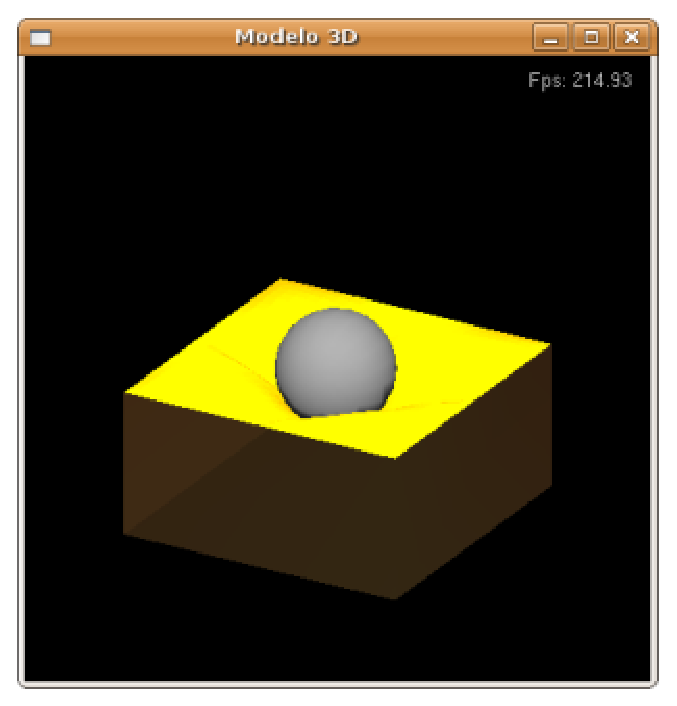
\includegraphics[]{Img/modeloPortada}
 \caption[Ejemplo del programa en ejecución]{Un ejemplo del modelo.}
 \label{programa:portada}
\end{figure}
\subsubsection{Constantes del experimento}
En una situación como la antes descrita hay muchísimas variables del modelo, sin embargo al momento de hacer la implementación en código decidí dejar fijas algunas de ellas, es decir que la única manera de cambiarlas es modificando en el código fuente y recompilando el programa por completo. Aquí está la lista de estas variables y su significado.

Primero las  variables del número de partículas que conforman el cuerpo flexible.

\begin{description}
 \item[LADO:] Número de partículas por lado del cuerpo flexible, y es la única variable independiente.
 \item[PARTICULAS:] Número total de partículas que forman el cuerpo flexible. Utilizamos $n^{2}$, en donde $n$ es LADO.
 \item[RESORTES:]Número de resortes que conectan el cuerpo flexible, es $2n(n - 1)$.
 \item[CUADROS:]Número total de caras que forman el cuerpo flexible, es igual a $(n - 1)^{2}$
\end{description}

Las variables que sirven para hacer la proyección ortogonal y poner el tope de las coordenadas del mundo son las siguientes:
\begin{description}
 \item[MUNDO:] Es el tope de las coordenadas del mundo.
 \item[FONDO:] Es el lugar donde se sitúa sobre el eje XZ, el fondo de la caja que forma el cuerpo flexible. Además de servir para otros cálculos dentro del programa, la única restricción es que su valor absoluto sea menor que MUNDO.
\end{description}

Una variable para integrar la ecuación de Newton 
\begin{description}
 \item[DT:] Es el tamaño del paso en el tiempo por cada vez que se integra la ecuación de Newton. Es decir es lo que en la parte de métodos numéricos llamé $\Delta t$.
\end{description}

\begin{description}
 \item[M:] Una única constante física, la masa de cada una de las partículas.
\end{description}
 
Los valores de estas constantes con las que se hizo este experimento están en la tabla~\ref{valores:constantes}.
\begin{table}
\ra{1.2}
\begin{center}
\begin{tabular} {@{}lrp{10cm}@{}}
\toprule
Constante & Valor & Comentario\\ 
\midrule
 LADO & 26 & Para que se vea mejor el modelo, se elige un número par\\
 PARTICULAS & 676 &  \\
 RESORTES & 1300 & \\
 CUADROS & 625 & \\ 
\midrule
 MUNDO & 100 & La proyección va de $-MUNDO$ a $MUNDO$ en cada eje\\
 FONDO & -50.0 & \\ 
\midrule 
 DT & 0.01 & \\ 
\midrule
 M & 0.009 & El peso total del cuerpo flexible es $M \cdot PARTICULAS$ \\
\bottomrule
\end{tabular}
\caption[Tabla con los valores de las constantes durante el experimento]{Valor de las constantes del experimento}
\label{valores:constantes}
\end{center}
\end{table}

\subsubsection{Variables del experimento}
La variables del experimento pueden ser modificadas en tiempo de ejecución por medio del menú que muestra en la figura~\ref{programa:menu}.

La primer categoría, \emph{Esfera}, se refiere al cuerpo rígido. En esta caso la esfera y la única variable que se puede modificar es su masa.

La categoría de \emph{Integrador}, se refiere el método numérico usado para integrar la ecuación de Newton, sólo se implementaron dos métodos el de Euler y el de Runge Kutta. Dado que cambiar de método a mitad de la simulación generalmente lleva a inestabilidad numérica, cada que se cambia el método, todos los objetos regresan a sus posiciones iniciales.

La categoría de variables físicas se refiere a los parámetros del cuerpo flexible que es posible cambiar. Se dividen en tres subcategorias una por cada fuerza que se acumula.

La presión del \emph{gas}, se puede prender o apagar por medio del checkbox. Además, se puede modular su magnitud variando el valor de la constante $k_{g}$, por medio del control.

La de la \emph{gravedad}, que al igual que la anterior se puede prender o apagar con el control y también se puede modular variando el valor de la constante $g$.

Por último la debida al \emph{resorte amortiguador}. Esta fuerza no se puede apagar, pero se puede variar por medio de la modificación de dos parámetros $k_{s}$, que, como ya se dijo, controla la rigidez del resorte y $k_{d}$ que controla el amortiguamiento o pérdida de energía debida al resorte.

\subsubsection{Opciones de visualización}
Hay otras opciones que se pueden modificar por medio del menú, que se refieren más a cómo se ve el modelo que a la física. Éstas se dividen en dos, las que controlan el render y las que controlan el flujo de la animación

Dentro de las del flujo de la animación, sólo hay dos controles, el de \emph{Iniciar/Pausar}, que mantiene la escena congelada cuando está marcado y el botón de \emph{Reiniciar}, que devuelve a todos los objetos a su posición original.

Dentro de la categoría de render, se encuentran los siguientes controles:

El \emph{wireframe}, si el checkbox está activado, sólo se pintarán las líneas del modelo, así se pueden apreciar todas las partículas que lo componen.

La \emph{luz}, dado que se utiliza una proyección ortogonal. La única fuente de profundidad viene de la luz y las sombras, Y el modelo contiene una única fuente de luz, localizada en $(0, k, 2k)$ en donde $k = MUNDO$. Con este control se puede prender o apagar esta fuente de luz.

La \emph{caja} que dice si se va a pintar o no las caras sólidas de la caja. Las caras sólidas se pintan con un cierto valor de transparencia, para que se aprecie mejor cómo se deforma la parte de abajo de la tela o cuerpo flexible.

Por último un par de controles que manejan el ángulo de rotación del modelo. Sólo se permite rotar sobre el eje $X$ o sobre el eje $Y$.

Los valores de default de estas variables (el valor que tiene al iniciar la ejecución) son los que muestra la tabla~\ref{valores:variables}.

\begin{figure}
 \centering
 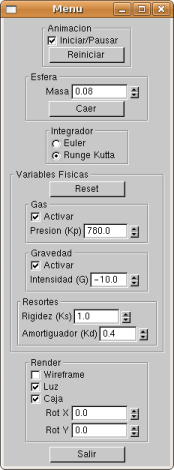
\includegraphics[]{Img/menu}
 \caption[Menú de usuario del programa]{Menú de usuario.}
 \label{programa:menu}
\end{figure}

\begin{table}
\ra{1.2}
\begin{center}
%\begin{tabular} {|c|c|p{10cm}|}
\begin{tabular} {@{}llp{10cm}@{}}
\toprule
Parametro & Valor & Comentario\\
\midrule
 Masa & 0.08 & Masa del cuerpo rígido \\
 Integrador & Runge Kutta & Método Numérico con el que se integra. \\
 Gas & Activado & El programa empieza con la fuerza del gas prendida \\
 $k_g$ & 780 & Constante de presión del gas \\
 Gravedad & Activada & La gravedad está activada \\
 $g$ & -10.0 & La gravedad es negativa (jala hacia abajo) \\
 $k_s$ & 1.0 & La fuerza de los resortes \\
 $k_d$ & 0.4 & El valor de damping \\
\bottomrule
\end{tabular}
\end{center}
\caption[Tabla con los valores de defecto de los parámetros]{Valor inicial de los parámetros del experimento}
\label{valores:variables}
\end{table}

\subsection{Características del entorno de pruebas}

\subsubsection{Software}

El programa fue hecho en su mayor parte en lenguaje C, el compilador elegido fue gcc por tratarse de un compilador libre y por ser el que se instala en la mayoría de las distribuciones de GNU/Linux (la gran mayoría de este trabajo fue desarrollado bajo este sistema operativo).

Sin embargo, al crear el menú de usuario fue necesario utilizar la biblioteca glui, que está escrita en objetos, por lo que al final se tuvo que compilar en C++, con el compilador g++.

Para poder compilar el código fuente de este programa es necesario tener un entorno de programación que contemple lo siguiente:

\begin{itemize}
 \item Un compilador de C++
 \item La biblioteca OpenGL
 \item La biblioteca glut
 \item La biblioteca glui
\end{itemize}

Todas éstas tienen alternativas libres, y además todas tienen la enorme ventaja de tener equivalentes en cualquier plataforma, por lo que si las bibliotecas están correctamente instaladas, debería de compilar el programa bajo cualquier sistema operativo.

Se ha hecho la prueba en los entornos GNU/Linux y Windows XP (en este último con el IDE Dev-C++, con un compilador Mingw).

\subsection{Hardware}
La mayoría de las pruebas fueron hechas en una estación de trabajo Sun Ultra 20, con las siguientes características.

\begin{itemize}
\label{maquina:trabajo} 
 \item Procesador: Opteron 1214 2.2GHz
 \item Memoria: 2GB DDR2
 \item Tarjeta de Video: Nvidia FX3500
 \item Acerleración gráfica: driver de nVidia
 \item Sistema Operativo: Ubuntu 7.04 64bits (kernell 2.6.20-16)
\end{itemize}

Esto no quiere decir que este sea el hardware mínimo, sólo que la \emph{mayoría} de las pruebas se realiaron en este hardware. Sin embargo, se ha ejecutado con éxito en equipos mucho más convencionales (las características de estos equipos así como su desempeño al ejecutar el programa se muestran más a detalle en la última sección de este capítulo).

\section{Ejemplos de las características físicas del modelo}
Para poner en evidencia ciertas características del modelo, se hicieron las siguientes pruebas sugeridas, la mayoría para probar la sensibilidad del programa ante la variacion de sus parámetros físicos.

\subsection{Probando la gravedad}
La gravedad es la única fuerza que actúa tanto en el cuerpo flexible como en en el cuerpo rígido. Para entender mejor cómo afecta se sugieren las siguientes pruebas.

Partiendo de los valores de \emph{\foreignlanguage{english}{default}}, se espera a que la tela se estabilice (figura \ref{programa:portada}). Ahora se \emph{aumenta} la gravedad a su valor más \emph{pequeño} (recordemos que hacer la gravedad más fuerte es hacerla más negativa), es decir, $g=$-12.0, se observa ahora como la gravedad es muy fuerte como para que la presión del gas infle la tela, por lo que queda colgando un poco. Las partículas que forman el cuerpo flexible son muy pesadas (son jaladas con más fuerza hacia abajo). Esta situación se muestra en la figura~\ref{grav:test1}. Ahora se deja caer la pelota y se espera que se estabilice de nuevo el programa, la gravedad hace que la pelota y las partículas pesen más, sin embargo la fuerza del gas que no se ha tocado compensa de alguna manera y no deja que se hunda más la pelota. Con la pelota estable sobre la tela, apagué la fuerza del gas. Al apagar la fuerza que equilibraba la gravedad todo se va hacia abajo, por la gravedad, pero como además esta fuerza es grande, la rigidez del resorte es poca para evitar un efecto de súper elongación como el que se ve en la figura~\ref{grav:test2}.

\begin{figure}
 \centering
 
\includegraphics[]{Img/modGra1}
 \caption[Ejecución con $g=$-12.0]{La gravedad aumenta a $g=$-12.0.}
 \label{grav:test1}
\end{figure}

\begin{figure}
 \centering
 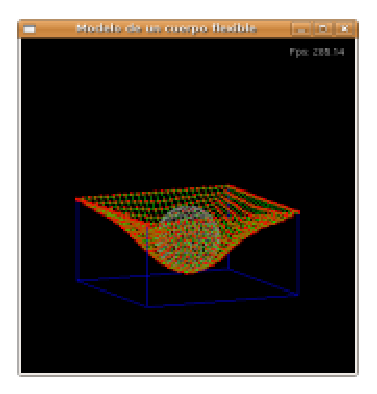
\includegraphics[]{Img/modGra2}
 \caption[Ejecución con fuerza de gravedad grande y sin presión]{La gravedad es grande y se apaga el gas.}
 \label{grav:test2}
\end{figure}

Reinicie la animación y vuelva a los valores de \emph{\foreignlanguage{english}{default}}. De nuevo espere a que se estabilice la tela ahora disminuya la gravedad a su máximo valor posible, es decir una gravedad positiva: $g=$1.0. Ahora verá que la tela se va más hacia arriba, como si se inflara más el cuerpo flexible, esto se debe a que ahora la gravedad no se opone a la presión del gas, sino mas bien le favorece, por lo que el cuerpo flexible, es jalado hacia arriba aún más, como se ve en la figura~\ref{grav:test3}. Ahora deje caer la pelota, como la gravedad es positiva y pequeña (su valor absoluto en una décima parte del valor normal) la pelota \emph{sube lentamente}, y se aleja del cuerpo flexible. La constante de gravedad influencía la velocidad de caída de los cuerpos.

\begin{figure}
 \centering
 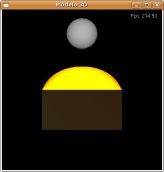
\includegraphics[]{Img/modGra3}
 \caption[Ejecución con la fuerza de gravedad apagada]{La gravedad es apagada.}
 \label{grav:test3}
\end{figure}

Por último vamos a reiniciar la animación y partiendo de los valores de \emph{\foreignlanguage{english}{default}} de los parámetros, se apaga la gravedad. Este comportamiento equivale a hacer $g=0$ con la diferencia de que se hacen menos cálculos, ahora vemos cómo de nuevo la tela se mueve hacia arriba, cómo la gravedad se oponía a la fuerza del gas y ya no está, el gas empuja la tela aún más hacia arriba. Si en esta situación se deja caer la pelota no pasará nada, debido a que la caída de la pelota \emph{depende de la gravedad}, y al no haber, simplemente no hay caída.

Si se apaga la gravedad después de dejar caer la esfera, ésta es empujada afuera del cuerpo flexible por un impulso.

\subsection{Probando la fuerza del gas}
Ahora se harán pruebas sobre la fuerza del gas. La fuerza del gas, por el diseño de nuestro experimento, se opone a la fuerza de gravedad, y actúa sólo sobre el cuerpo flexible, sin embargo tiene cierto efecto sobre la velocidad de las partículas del cuerpo flexible, que a su vez tienen cierto efecto sobre el cuerpo \emph{rígido} al momento de la colisión.

Inicie el programa con los valores de \emph{\foreignlanguage{english}{default}}, ahora apague la fuerza del gas y espere a que se estabilice el modelo, como se ve el la figura~\ref{pres:test1}. Como no hay fuerza del gas, la tela o cuerpo flexible cuelga agarrada de las orillas de la caja. Ahora deje caer la pelota sobre el cuerpo flexible y espere a que se estabilice la animación, justo como se ve en la figura~\ref{pres:test2}. Prenda la fuerza del gas y observe como la pelota es lanzada hacia arriba súbitamente como se ve en la figura~\ref{pres:test3}.

\begin{figure}
 \centering
 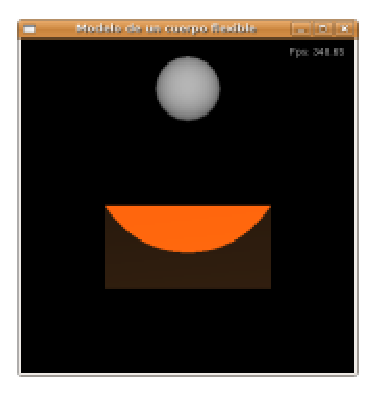
\includegraphics[]{Img/modPres1}
 \caption[Ejecución con la fuerza del gas apagada]{Fuerza del gas apagada.}
 \label{pres:test1}
\end{figure}

\begin{figure}
 \centering
 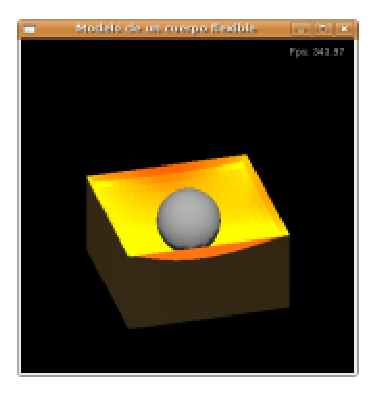
\includegraphics[]{Img/modPres2}
 \caption[Ejecución con la esfera cayendo en ausencia de fuerza del gas]{La pelota cae mientras está apagado el gas.}
 \label{pres:test2}
\end{figure}

\begin{figure}
 \centering
 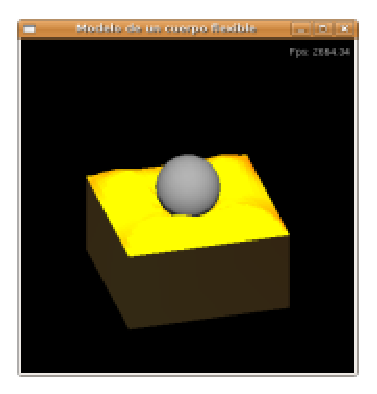
\includegraphics[]{Img/modPres3}
 \caption[Ejecución con la esfera lanzada por la fuerza del gas]{La pelota es lanzada por la fuerza del gas.}
 \label{pres:test3}
\end{figure}

Otra prueba es ver los efectos de la variación de la constante $k_g$. Inicie la animación con los valores de \emph{\foreignlanguage{english}{default}} y haga la constante $k_g$ pequeña, por ejemplo $k_g =$ 350.0; verá cómo el gas no es lo suficientemente fuerte para inflar el cuerpo flexible. Ahora aumente poco a poco la constante $k_g$ y observe cómo se infla cada vez más el cuerpo flexible. En la figura~\ref{pres:test4} se ilustran estas situaciones para diferentes valores en aumento de la constante $k_g$.

\begin{figure}
 \centering
 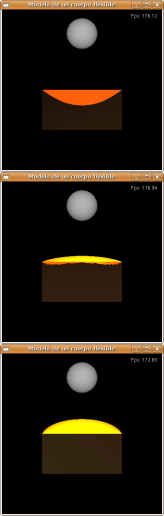
\includegraphics[]{Img/modPres4}
 \caption[Ejecución con diferentes valores de la constante de gas]{Variando la fuerza del gas: $k_g=$350.0 (arriba), $k_g=$730.0 (centro), $k_g=$970.0 (abajo)}
 \label{pres:test4}
\end{figure}

\subsection{Probando los resortes amortiguadores}
La siguientes pruebas sirven para mostrar cómo funcionan los resortes amortiguadores. Primero vamos a hacer una prueba con la constante de \emph{\foreignlanguage{english}{damping}} $k_d$. Como ya se dijo, el damping es una forma de perder energía del sistema y, por lo tanto, de eventualmente estabilizarse. Iniciemos la animación con los valores de \emph{\foreignlanguage{english}{default}} y hagamos la constante $k_d=0$, es decir quitemos todo el \emph{\foreignlanguage{english}{damping}}. Vemos que la tela empieza a oscilar rápidamente como consecuencia del gas. Ahora quitemos también el gas y esperemos un momento; veremos como la tela oscila sin detenerse ni estabilizarse en ningún momento, es cierto que cada vez oscila menos, pero ciertamente tardará mucho en detenerse (o nunca se detendrá).

En la figura~\ref{res:test1}, podemos ver diferentes oscilaciones sin control por falta de un amortiguador. Como ya se había dicho, el amortiguador agrega realismo (en la total ausencia de \emph{\foreignlanguage{english}{damping}}, el cuerpo flexible se ve poco real). La contra parte es que a mayor \emph{\foreignlanguage{english}{damping}}, también hay menos estabilidad numérica, por lo que el modelo es sumamente sensible al aumento en este parámetro.

Podemos ir aumentando el valor de $k_d$ poco a poco y ver cómo el modelo se vuelve inestable, podemos por ejemplo poner el máximo posible $k_d=$0.6 y reiniciar la animación, esperar a que se estabilice y apagar el gas, el modelo explota (ver figura~\ref{res:test4}).

Ahora analicemos la constante de rigidez $k_s$. Esta constante hace a los resortes más poderosos, por lo que en general hace que las partículas que están unidas por ellos, se separen menos, es decir hace más estable el cuerpo flexible en general, además de prevenir el efecto de super elongación.

Iniciamos la animación con los valores de default y pongamos la constante del resorte $k_s$ a su máximo valor. Ahora apaguemos el gas y vemos como la caída de la tela es menor, sin embargo al apagar y prender varias veces el gas también nos damos cuenta de que el cuerpo flexible parece oscilar más, como consecuencia de que los resortes en general jalan más fuerte, tanto hacia arriba como hacia abajo.

Ahora con la constante $k_s$ en el máximo y el gas prendido, vayamos poco a poco subiendo la presión del gas, aumentando $k_g$ hasta su máximo $k_g=$2000.0. Podemos ver cómo aun llegando al máximo de $k_g$, el cuerpo flexible se expande poco; esperemos a que se estabilice, como se ve en la figura~\ref{res:test5}. Ahora que tenemos el modelo estable y con ambas constantes $k_s$ y $k_g$ al máximo, poco a poco vayamos haciendo $k_s$ más pequeña y podremos apreciar como el cuerpo parece inflarse más (la resistencia de la membrana que lo mantiene unido es menor), como se ve en la figura~\ref{res:test6}, hasta llegar al momento donde explota ($k_s$ = 0.0).

\begin{figure}
 \centering
 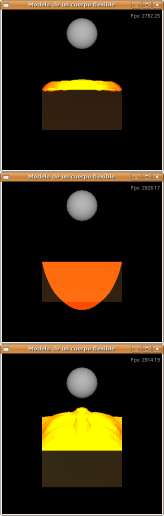
\includegraphics[]{Img/modRes1}
 \caption[Ejecución sin fuerza de amortiguamiento]{Oscilación sin control: $k_d$=0.0}
 \label{res:test1}
\end{figure}

\begin{figure}
 \centering
 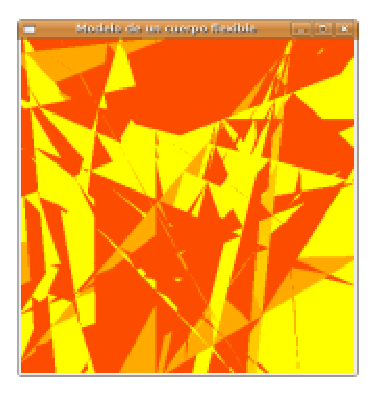
\includegraphics[]{Img/modRes4}
 \caption[Explosión por inestabilidad numérica]{La animación explota por inestabilidad numérica}
 \label{res:test4}
\end{figure}

\begin{figure}
 \centering
 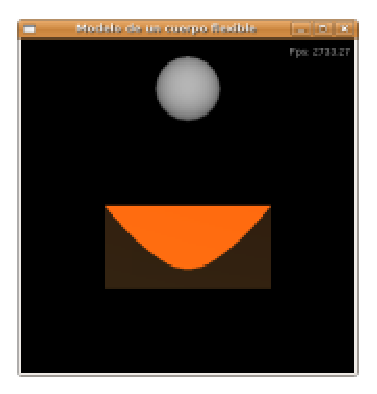
\includegraphics[]{Img/modRes5}
 \caption[Ejecución con fuerza del gas y rigidez al máximo]{El gas está al máximo $k_g=$2000.0 al igual que la rigidez de los resortes $k_s=$2.0}
 \label{res:test5}
\end{figure}

\begin{figure}
 \centering
 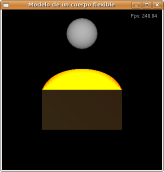
\includegraphics[]{Img/modRes6}
 \caption[Ejecución con fuerza del gas y rigidez pequeña]{El cuerpo flexible se infla como consecuencia del gas la máximo y $k_s$ pequeña}
 \label{res:test6}
\end{figure}

\section{Presentación de resultados}

Una manera de medir la eficiencia tanto de la implementación como del modelo es ver cuánto se tarda en hacer los cálculos el programa antes de pintar un frame. Esta medida de rendimiento es calculada comúnmente en las simulaciones gráficas y por ello me decidí a implementarla. Como ya se dijo, esto es dependiente del hardware, así que aquí presento dos tipos de análisis.

En la primera parte, se deja como constante el hardware, hago las pruebas en la misma computadora y se varían los cálculos que se hacen en la ejecución del programa.

En la segunda parte se mantienen constantes los cálculos en el programa y se ejecuta en varios ambientes de pruebas (diferentes máquinas y distintos sistemas operativos).

\subsection{Desempeño del programa}

La medida mas comúnmente usada es el número de cuadros que la aplicación pinta en un segundo o fps (de abreviar en inglés \emph{\foreignlanguage{english}{frames per second}}). La rutina que calcula los fps se implementó con el siguiente código dentro de la función con el registro de callback idle.

\begin{verbatim}
frame++;
time = glutGet(GLUT_ELAPSED_TIME);
if (time - timebase > 1000) {
  fps = frame * 1000.0 / (time - timebase);
  timebase = time;
  frame = 0;
}\end{verbatim}

En donde la variable global \verb|frame|, ya fue inicializada la primera vez en ceros. Esta rutina mide los frames por segundo, que después son desplegados en la parte superior izquierda de la pantalla.

Estas pruebas fueron realizadas en la máquina ya descrita antes en la sección~\ref{maquina:trabajo}.

Las variantes consideradas son las siguientes:

\begin{description}
 \item[Estado de la animación:]la animación puede estar en pausa o en movimiento, cuando está en pausa, se pueden cambiar la opciones de render y de la rotación de la cámara, pero el programa deja de hacer los cálculos del método numérico y por ende de la acumulación de fuerzas.
 \item[Hay colisiones:]la rutina de detección de colisiones siempre es ejecutada, sin embargo sólo en caso de que se detecte una colisión se llama a la rutina de respuesta de las colisiones.
 \item[Método Numérico:]el programa ejecuta uno de dos métodos numéricos para calcular el estado siguiente de la animación, puede ser por Euler o por Runge Kutta, de donde este último requiere de casi cuatro veces mas cálculos.
 \item[Fuerza del gas:]calcular la fuerza del gas requiere de hacer cálculos sobre el área y el volumen del cuerpo flexible, cuando esta fuerza está apagada, los cálculos se omiten.
 \item[Opciones de \emph{\foreignlanguage{english}{render}}:]las opciones del \emph{\foreignlanguage{english}{render}} hacen que se tengan que hacer cálculos de la iluminación y dar color a los objetos con base a dichos cálculos.
\end{description}

La nomenclatura de la prueba usando estas variables se especifica en el cuadro~\ref{nomenclatura:prueba}.

Cada una de las variantes arriba mencionadas puede tener dos valores. El \emph{\foreignlanguage{english}{render}} puede tener muchos valores pero para hacer las pruebas sólo voy a considerar dos: prendido, cuando se dibujan todos los cuerpos en estado sólido con iluminación y apagado, cuando se dibuja en wireframe sin luz y no se dibuja la caja del cuerpo flexible.

\begin{table}
\ra{1.2}
\begin{center}
\begin{tabular} {@{}llp{10cm}@{}}
\toprule
 Variable & Valores & Explicación\\
\midrule 
 Animación & 0 ó 1 & Se considera 1 cuando la animación esta en marcha, y 0 cuando está en pausa. \\
 Colisiones & 0 ó 1 & Se considera 1 cuando hay una colisión y se ejecuta la respuesta, 0 cuando no hay colisión y sólo se ejecuta la detección. \\
 Método Numérico & 0 ó 1 & Se considera 1 cuando se ejecuta Runge Kutta y 0 cuando se ejecuta Euler. \\
 Fuerza del gas & 0 ó 1 & Se considera 1 cuando está prendida y 0 cuando está apagada. \\
 Render & 0 ó 1 & Se considera 1 cuando se hace la mayor cantidad render, como se explicó arriba y 0 cuando se hace el mínimo posible. \\
\bottomrule
\end{tabular}
\end{center}
\caption[Explicación de la nomenclatura de la prueba del programa]{Nomenclatura de la prueba}
\label{nomenclatura:prueba}
\end{table}

Se tienen pues cinco posibles variantes, cada una con dos valores. Se ejecutaron los 18 casos posibles (la animacion apagada implica que haya opciones que no tengan sentido, por eso son sólo 18 en vez de 32) y para cada caso anoté entre qué valores oscilan los fps. Los resultados se resumen en la tabla~\ref{resultado:prueba1}.

La razon por la cual los fps, son un rango es que al momento de la ejecución, cada segundo varía el valor de los fps. Es por eso que al hacer el experimento con las condiciones de cada caso, anote tanto el valor máximo que alcanzaron lo fps, como el valor mínimo; esto es lo que llamo el rango.

La columna de contribución, representa cuánto contribuye a los cálculos la prueba en cuestión con respecto a que se hacen \emph{todos} los cálculos, tomando como base el caso en que todas las variables están prendidas. La contribución $C$ es calculada de la siguiente manera:

$$ C = \frac{FPS_{min} + FPS_{max}}{2} \div FPS_{base}$$

En donde $FPS_{min}$ es el mínimo de fps en cada categoría y $FPS_{max}$ es el máximo de fps en la misma, $FPS_{base}$ es el promedio de fps de la categoría base, para este caso $FPS_{base} =$ 210.81 dado que es el promedio de los $FPS$ de la prueba que más poder requiere y se presenta en el último renglón de la tabla.

\begin{table}
\ra{1.2}
\begin{center}
%\begin{tabular} {|c|c|c|c|c|c|c|}
\begin{tabular} {@{}cccccrr@{}}
\toprule
 Anim & Coli & Método & F. Gas & Render & FPS & Contr\\
\midrule
 0 & n/a & n/a & n/a & 0 & 2753.08 - 2768.15 & 0.08\\
 0 & n/a & n/a & n/a & 1 & 2754.01 - 2826.18 & 0.08\\
 1 & 0 & 0 & 0 & 0 & 654.35 - 663.34 & 0.32\\
 1 & 0 & 0 & 0 & 1 & 620.38 - 630.37 & 0.34\\
 1 & 0 & 0 & 1 & 0 & 501.04 - 512.98 & 0.42\\
 1 & 0 & 0 & 1 & 1 & 464.03 - 491.02 & 0.44\\
 1 & 0 & 1 & 0 & 0 & 447.99 - 456.54 & 0.47\\
 1 & 0 & 1 & 0 & 1 & 454.09 - 474.05 & 0.45\\
 1 & 0 & 1 & 1 & 0 & 240.52 - 251.99 & 0.86\\
 1 & 0 & 1 & 1 & 1 & 203.57 - 212.57 & 1.01\\
 1 & 1 & 0 & 0 & 0 & 640.72 - 660.54 & 0.32\\
 1 & 1 & 0 & 0 & 1 & 612.76 - 627.74 & 0.34\\
 1 & 1 & 0 & 1 & 0 & 499.03 - 512.03 & 0.42\\
 1 & 1 & 0 & 1 & 1 & 470.06 - 484.52 & 0.44\\
 1 & 1 & 1 & 0 & 0 & 347.31 - 357.29 & 0.60\\
 1 & 1 & 1 & 0 & 1 & 333.67 - 342.32 & 0.62\\
 1 & 1 & 1 & 1 & 0 & 214.34 - 219.26 & 0.97\\
 1 & 1 & 1 & 1 & 1 & 209.04 - 212.57 & 1.00\\
\bottomrule
\end{tabular}
\end{center}
\caption[Resultados de la prueba del programa]{Resultados primera prueba}
\label{resultado:prueba1}
\end{table}

Hay algunos datos interesantes con respecto a la tabla \ref{resultado:prueba1}, por ejemplo el hecho de lo poco que contribuye el render al desempeño de la animación (el .03). Esto se explica por que cuando el render está apagado se trazan más objetos gráficos, se dibujan cuatro lineas y cuatro puntos por cada cara, mientras que cuando el render está prendido si bien se hacen cálculos de iluminación sólo se dibuja un cuadro por cada cara.

También de la tabla, puedo concluir  que lo que más contribuye al desempeño de la animación es el método numérico usado, pues como dijimos el
método de RK4, lleva casi cuatro veces más cálculos que el método de Euler (en la tabla se ve que representa el .56 de los cálculos).

El otro factor que hace considerablemente más lenta la animación es el cálculo de la fuerza del gas con el .48 del tiempo.

\subsection{Desempeño del programa en diferentes ambientes}

La última prueba consistió en hacer constante la ejecución del programa y ver qué desempeño tiene en diferentes tipos de hardware.

Para esta  prueba se ejecutó el programa en diferentes ambientes. En cada ambiente se consideran importantes sólo las siguientes características: la memoria principal, el sistema operativo, el procesador, la arquitectura y si hay o no memoria de vídeo.

La ejecución del programa se hizo de una manera típica, lo que haciendo una equivalencia con la prueba anterior es que esté en marcha la animación, que haya colisiones con el método de Runge Kutta, que haya fuerza del gas y que el \emph{\foreignlanguage{english}{render}} se haga completo. También se hizo la ejecución con las siguientes características mínimas: método de Euler y sin fuerza de gas. De ambas pruebas se miden los fps.

Los resultados se listan a continuación.
\begin{itemize}
 \item Sistema Operativo: Ubuntu 7.04
 \item Procesador: Opteron 1214 a 2.2GHz
 \item Memoria RAM: 2.0GB
 \item Memoria de Video: Tarjeta Nvidia FX3500, 256MB, driver propietario
 \item Velocidad en prueba mínima: 612.76 - 627.74fps
 \item Velocidad en prueba normal: 209.04 - 212.57fps
\end{itemize}

\begin{itemize}
 \item Sistema Operativo: Windows XP professional edition
 \item Procesador: AMD Duron a 1.2GHz
 \item Memoria RAM: 512MB
 \item Memoria de Video: Tarjeta Nvidia 64MB
 \item Velocidad en prueba mínima: 72.0 - 102.0fps
 \item Velocidad en prueba normal: 60.0 - 94.0fps
\end{itemize}

La última prueba se llevó a cabo en una máquina virtual, con el fin de evaluar los requerimientos mínimos.

\begin{itemize}
 \item Sistema Operativo: Windows XP professional edition
 \item Procesador: Dual Core AMD Opteron 999Mhz
 \item Memoria RAM: 256MB
 \item Memoria de Video: Ninguna, adaptador VM-Ware SVG 2
 \item Velocidad en prueba mínima: 65.40 - 71.72fps
 \item Velocidad en prueba normal: 46.44 - 52.22 fps
\end{itemize}



\chapter*{Conclusiones}
\addcontentsline{toc}{chapter}{\numberline{}Conclusiones}
\markboth{CONCLUSIONES}{CONCLUSIONES}

Después de haber hecho pruebas y evaluado los resultados obtenidos presento las siguientes conclusiones.

La más importante: las ecuaciones diferenciales, permiten modelar gráficamente el comportamiento físico de un cuerpo neumático que interactúa con un cuerpo rigido en tiempo real.
También hay que recalcar que este modelo tiene sustento en la física. 
Es decir es un modelo basado en física y no en geometría.

Creo también que la técnica aquí usada; la de utilizar un gas ideal dentro del cuerpo flexible, es muy buena para enfrentar este tipo de problemas.
La técnica nos porporciona todo lo que desearíamos para hacer una animación: es computacionalmente barata; al menos lo suficiente para alcanzar tiempo real, y es físicamente adecuada para modelar el gas.

La implementación como se describe, depende poco del poder gráfico.
El render sigue siendo una operación relativamente barata \emph{en comparación} con los cálculos numéricos.
Dentro de los cálculos numéricos, lo que más contribuye es el método numérico de Runge Kutta seguido de la acumulación de la fuerza del gas.

Si bien el utilizar el método de Euler hace considerablemente más rápido de ejecutarse el programa, recomiendo usar el método de Runge Kutta.
Esto ofrece una mayor estabilidad ante la variación de las constantes, lo que se traduce en la posibilidad de una mejor interacción.
También creo que este método no es tan complejo de implementar.

El \emph{\textenglish{damping}} es un parámetro que debe de estar presente. 
Sin embargo, requiere tener mucho cuidado al determinar un valor adecuado.
Considero que el valor más adecuado es el más grande posible sin que la animación explote.
Este modelo es muy sensible a las variaciones (incluso \emph{pequeñas}) de éste parámetro.

Se recomienda ampliamente que al momento de programar se tome tiempo para hacer una adecuada elección de las estructuras de datos.
Guardar todo en una estructura de datos lineal simplifica bastante la programación.
De igual manera, recomiendo tener diferentes maneras de acceder a las propiedades de las partículas, ya sea por los resortes o por medio de las caras.

El modelo del gas ideal es un modelo muy recomendado para simular cuerpos flexibles.
Con una adecuada elección de los parámetros se puede tener un comportamiento bastante realista.
Por lo que considero que el objetivo fundamental de este trabajo se cumple.

Hay muchas mejoras posibles para esta implementación, pienso que hay campo para futuras investigaciones en los siguientes detalles:

\begin{itemize}
 \item Investigar sobre un método numérico más eficiente, aquel que dé más rapidez sin perder estabilidad.
 \item El manejo de colisiones más eficiente.
\end{itemize}

Para el método numérico se hicieron pruebas con el integrador de Verlet.
Sin embargo, abandoné ese camino porque en un esquema como ése no se toma en cuenta la velocidad de la partícula.
Por lo que no encontré manera de responder a las colisiones.
Creo que investigar la manera de incluir una fuerza de impulso como respuesta a la colisión y utilizar el integrador de Verlet daría resultado.

Hay también que considerar una respuesta a las colisiones que conlleve una pérdida de energía al momento de la colisión.
Es decir, eliminar el supuesto de colisiones perfectamente elásticas.
Aunque escribí en el segundo capítulo sobre ellas, no fueron implementadas en el programa.

Mi forma de manejar tanto la detección como la respuesta de las colisiones  no es la más eficiente, pues pruebo una a una las partículas del cuerpo flexible.
Algúna estructura de datos geométrica (como un \emph{\textenglish{octree}} o un \emph{\textenglish{range tree})} que probara sólo las partículas cercanas haría mejor la detección.

También hay una mejora posible si se considera que el cuerpo flexible puede colisionarse consigo mismo. 
Es decir, probar colisiones de las caras del cuerpo con cada una de las partículas y luego responderlas.
Considero que en cualquier configuración del cuerpo flexible que no sea un volumen convexo éste problema estará presente.


\chapter{Sobre el software libre}
Un objetivo secundario cuando empecé a hacer esta tesis, fue que toda ella fuera hecha con Software Libre. Al final tengo que admitir que esto no fue llevado a cabo por completo, pues todas las figuras del primer capítulo con la excepción de la~\ref{OsciAmor:fig} fueron hechas en AutoCAD (http://www.autodesk.es).

Aun así, pienso que este objetivo se cumplió parcialmente, pues fuera de lo antes mencionado todo se hizo en Software Libre; el desarrollo del programa fue hecha sobre GNU/Linux en particular sobre la distribución Ubuntu (www.ubuntu.com).

Para programar se utilizó gcc (http://gcc.gnu.org/), junto con Mesa (http://www.mesa3d.org/) y freeglut (http://freeglut.sourceforge.net/), la biblioteca glui (http://www.cs.unc.edu/rademach/glui/) también es software libre. Como IDE utilice Geany (http://geany.uvena.de/) y debo decir que estoy muy satisfecho con él.

Cuando hubo necesidad de hacer pruebas en Windows, también se ocuparon programas libres: se compiló con Dev-C++ (http://www.bloodshed.net/devcpp.html) como IDE y con Migwn (http://www.mingw.org/) como compilador junto con glui y freeglut.

El texto de la tesis se escribió en \LaTeX, en Ubuntu utilice tetex (http://web.bilkent.edu.tr/History/valley/tetex-index.html)y en Windows miktex (http://miktex.org/).

También fue de muchísima ayuda contar con un repositorio para guardar los avances del proyecto, esto me dio la enorme ventaja de poder trabajar en cualquier computadora que tuviera acceso a internet. Para eso se hizo uso de apache (http://www.apache.org/) y de subversion (http://subversion.tigris.org/).


%\bibliographystyle{ieee_esp}
\nocite{*} %Print the whole bibliography even the entries not explicitly cited in text

\printbibliography

\addcontentsline{toc}{chapter}{\bibname}

\end{document}
